\setchapterpreamble[u]{\margintoc}
\glsresetall % reset glossary
\chapter{Optimizing modular structures}
Introduction TODO

In \secref{sec:05_01}, we provide a detailed explanation of the modifications needed to apply modular constraints to the \gls{tto}. Specifically, we focus on how to model the problem when multiple modules are used and how topological buckling constraints are implemented in modular structures. Finally, in \secref{sec:05_02}, we evaluate the proposed formulation through various 2D and 3D test cases, aiming to gain a better understanding of modular structures.
\marginnote{Part of the content presented in this chapter has been published and showcased during a conference as:\\Stragiotti, E. et al. (2022) "Enhanced truss topology optimization ({TTO}) applied to a cellular wing box", in \textit{ASMO-UK 12, an ISSMO Conference on Engineering Design Optimization}. Book of proceedings. Leeds, United Kingdom~\cite{stragiotti_enhanced_2022}.}
\section{Formulation of a modular structure optimization algorithm} \label{sec:05_01}
Assembled modular ultralight structures present an opportunity to greatly improve the performance and cost efficiency of modern aerostructures~\sidecite{cramer_elastic_2019}. The repetitive nature brings various interesting features among which reduced tooling, fast assembly, and short repair time. Additionally, as the mechanical performance of the structure is greatly influenced by the topology and the materials of the repetitive pattern, modular structures are naturally prone to optimization.

In the field of structure optimization, periodic materials are often modeled through asymptotic homogenization~\sidecite{zhou_design_2008}. The heterogeneous module topology (also called \gls{rve}) is treated as homogeneous material with associated mechanical properties \ie equivalent elastic tensor, shear modulus, etc. The homogenization approach is valid only if the \gls{rve} contains enough information about the heterogeneous material and if the structure presents significant periodicity~\sidecite{kalamkarov_asymptotic_2009,li_anisotropic_2020}. 

Nevertheless, our work pertains to structures that frequently exhibit one or more dimensions significantly smaller than the remaining dimensions, such as the thickness of a wingbox or a sandwich panel. In the context of designing modular structures (and not materials), no scale separation is assumed between the repetitive pattern and the structure itself. Consequently, the assumptions of asymptotic homogenization are not always verified. To address this, full-scale approaches~\sidecite{wu_topology_2021} have been developed.

\subsection{Variable linking}
\begin{figure*}
    \centering
    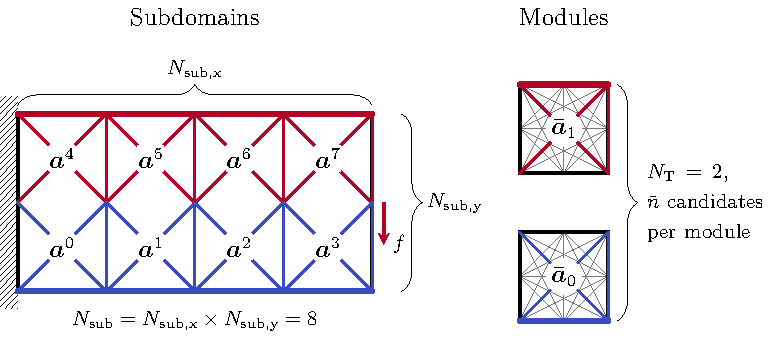
\includegraphics{figures/05_cellular_opt/00_modules_VL_bc/modules_bc.pdf}
    \caption{Notations used for the definition of the variable linking approach used to apply the modularity constraints.}
    \label{fig:05_VL}
\end{figure*}

The variable linking approach~\sidecite{zhang_scale-related_2006} is a full-scale optimization technique that involves first dividing a structure into several subdomains, which are connected in the optimization process -- \ie subdomains that belong to the same module all share the same cross-sectional areas. The primary goal is to make the manufacturing phase simpler and more efficient, allowing to assembly of big structures starting from smaller repetitive modules. With this approach, the optimization perspective shifts. The optimizer design space using the variable linking approach is restricted to the optimization of the topology of the modules, using the whole structure just to evaluate and impose the necessary mechanical constraints.

We use \figref{fig:05_VL} to illustrate the notation employed in this thesis for modular structures. On the left-hand side of the image, we have the whole test case that we aim to optimize, which is divided into $N_\text{sub}$ subdomains. Each of these subdomains is bound to exhibit the topology of one of the $N_\text{T}$ module topologies presented on the right side of the image. It is assumed for simplicity that each module has the same external shape and an identical ground structure used for discretizing the module volume. Within this framework, $\bar{n}$ represents the number of candidate bars in one module, and if we assume a fully connected mesh, we can define $\bar{n} = \bar{m} \cdot (\bar{m}-1)/2$, where $\bar{m}$ stands for the number of nodes in the module. Consequently, for the overall structure, we can write the relationship $N_{\text{el}} = N_{\text{sub}}\bar{n}$.

The vector that holds all the cross-sectional areas of the modules is represented by $\bar{\vect{a}}$, and it belongs to the set of positive real numbers $\mathbb{R}_+^{N_\text{T} \cdot \bar{n}}$. This vector is essentially a grouping of individual cross-sectional areas $\bar{\vect{a}}_t$ for each of the $N_\text{T}$ modules. In mathematical terms, $\bar{\vect{a}}$ is defined as follows:
\begin{equation}
    \bar{\vect{a}} :=  \{ \bar{\vect{a}}_t \in \mathbb{R}_+^{\bar{n}} \;|\; \forall t \in [1,\dots,N_\text{T}]\}
\end{equation}

The topology of the entire structure $\vect{a}$, which originates from the submodules' topology $\bar{\vect{a}}$, is the assembly of the individual cross-sectional areas of every one of the $N_{\text{sub}}$ subdomains and is defined as follows:
\begin{equation}
    \vect{a} :=  \{\vect{a}^j \;|\; \forall j \in [1,\dots,N_{\text{sub}}]\}
\end{equation}
and is evaluated using:
\begin{equation}
    \vect{a} = \sum_{t=1}^{N_\text{T}} \vect{h}_t\otimes\bar{\vect{a}}_t = \sum_{t=1}^{N_\text{T}} \begin{bmatrix}
        h_{1,t} \: \bar{\vect{a}}_t \\
        \vdots\\
        h_{N_{\text{sub}},t} \: \bar{\vect{a}}_t 
        \end{bmatrix}
        \label{eq:05_VL}
\end{equation}
where the $\otimes$ operator represents the Kronecher product and $\vect{h}_{t}$ is the $t$-th column of the module mapping matrix $\matr{H} = [\vect{h}_0,\dots,\vect{h}_{N_\text{T}}] \in \mathbb{B}^{N_{\text{sub}},N_\text{T}}$, where $\mathbb{B}=\lbrace 0,1 \rbrace$ is the Boolean domain. $h_{j,t}$ is the element at the $j$-th row and $t$-th column of the matrix $\matr{H}$. The module mapping matrix $\matr{H}$ indexes are defined as follows:
\marginnote{In the case of the structure shown in \figref{fig:05_VL} we have:
\begin{equation}
    \matr{H}=
\begin{bNiceMatrix}[first-row,last-col]
    \scriptstyle\textcolor{axis_gray}{t=0} &\scriptstyle\textcolor{axis_gray}{t=1}&  \\
    1 & 0 & \scriptstyle\textcolor{axis_gray}{\,j=0} \\
    1 & 0 & \scriptstyle\textcolor{axis_gray}{\,j=1} \\
    1 & 0 & \scriptstyle\textcolor{axis_gray}{\,j=2} \\
    1 & 0 & \scriptstyle\textcolor{axis_gray}{\,j=3} \\
    0 & 1 & \scriptstyle\textcolor{axis_gray}{\,j=4} \\
    0 & 1 & \scriptstyle\textcolor{axis_gray}{\,j=5} \\
    0 & 1 & \scriptstyle\textcolor{axis_gray}{\,j=6} \\
    0 & 1 & \scriptstyle\textcolor{axis_gray}{\,j=7} 
\end{bNiceMatrix}
\end{equation}
as the lower submodules (numbered from 0 to 3) exhibit the topology of module $t=0$, while the upper submodules (numbered 4 to 7) the topology of module $t=1$.}
\begin{equation}
    h_{j,t} =
    \begin{cases}
      1 & \text{if the $j$-th subdomain presents the topology of the $t$-th module,} \\
      0 & \text{otherwise.} 
    \end{cases}
\end{equation}
Lastly, we introduce some notation to denote specific bars within the modules and subdomains. We represent the cross-sectional area of the $i$-th bar of the $t$-th module as $\bar{\vect{a}}_{t,i}$, while the cross-sectional area of the $i$-th bar of the $j$-th subdomain as $\vect{a}^j_i$.
\subsection{Topological buckling of modular structures}
Addressing topological buckling in modular structures is a more complex task compared to monolithic structures. This complexity arises from the fact that we must not only consider bars within a single module's design space but also those connecting different modules. Since the nature of this problem heavily relies on how the modules are arranged within the structure, we have opted for a simplification. \marginnote{
\eqref{eq:04_chain_len}:
\begin{equation*}
    \ell^*_i(\vect{a}):= 
    \begin{cases}
        \ell_i & \text { if } i \notin \mathcal{C}_{l,r}(\vect{a}) \\
        \sum \ell_{r} \;|\; r \in \mathcal{C}_{l,r}(\vect{a})  & \text { otherwise.}
    \end{cases}
\end{equation*}
\eqref{eq:04_side_cons_chain}: 
\begin{equation*}
    a_{r}\geq a_{r=1}, \; r \in \mathcal{C}_{l,r}(\vect{a}), \; \forall r \neq 1.
\end{equation*}
} We focus only on the assessment of nodal instability within each module, modifying the length $\ell^*$ used to evaluate the critical buckling force of \eqrefnotext{eq:04_buck} and \eqref{eq:04_chain_len} only of compressive chains of bars that fall inside a module. Additionally, \eqref{eq:04_side_cons_chain} is modified as follows:
\begin{equation}\label{eq:05_side_cons_chain_modular}
    \bar{\vect{a}}_{t,r} \geq \bar{a}_{t,r=1} \quad r \in \mathcal{C}_{l,r}(\bar{\vect{a}}_t) \quad \forall t \in [1,\dots,N_\text{T}].
\end{equation}
We have made this choice knowing that the high connectivity of modular structures tends to reduce the occurrence of nodal instability within the structure. Any potential nodal instability in compressive chains at the structure level is addressed in a subsequent post-processing phase.

\subsection{Optimization formulation}
The monolithic formulation \ref{eq:04_optim_complete} is updated using \eqsref{eq:05_VL} and \eqrefnotext{eq:05_side_cons_chain_modular} to obtain the modular optimization formulation \ref{eq:05_optim_complete_modular} that use the variable linking approach. Formulation~\ref{eq:05_optim_complete_modular} is stated in terms of modular cross-sectional areas $\bar{\vect{a}}$, member forces $\vect{q}$ and nodal displacements $\vect{U}$ as follows:
\begin{equation}
    \begin{aligned}
    \min_{\bar{\vect{a}}, \vect{q}, \vect{U}}   && V &= \vect{\ell}^{T}\vect{a}\\
    \textrm{s.t.}  && \vect{a} &= \sum_{t=1}^{N_\text{T}} \vect{h}_t\otimes\bar{\vect{a}}_t \\ 
    && \matr{B}\vect{q} &= \vect{f} && \\
    && \vect{q} &= \frac{\vect{a}E}{\vect{\ell}}\vect{b}^T\vect{U} &&  \\
    && \vect{q} &\geq -\frac{s\vect{a}^2}{\vect{\ell}^{*2}} &&  \\
    && -\sigma_c\vect{a} &\leq \vect{q} \leq \sigma_t\vect{a} &&  \\
    && \bar{\vect{a}}_{t,r}&\geq \bar{a}_{t,r=1} && r \in \mathcal{C}_{l,r}(\bar{\vect{a}}_t),\, \forall t \\
    && 0 &\leq \bar{\vect{a}} \leq \frac{4 \pi \bar{\vect{\ell}}^2}{\lambda_{\text{max}}}, \\
    \end{aligned}
    \tag{${\mathbb{M}}_\text{1}$}
    \label{eq:05_optim_complete_modular}
\end{equation}
where $\bar{\vect{\ell}}$ represents the vector of the lengths of the bars within the modules.

The total number of design variables in the formulation is expressed as $N_\text{T}\bar{n} + N_{\text{sub}}\bar{n} + 2M$ or $N_\text{T}\bar{n} + N_{\text{sub}}\bar{n} + 3M$, depending on whether the test case is two or three-dimensional. The number of constraints is, however, equal to the monolithic optimization. This fact arises due to the localized nature of stress, buckling, and compatibility constraints, which are all referenced not only to individual modules but to the entire structure.

The formulation is solved by reusing the proposed two-step optimization algorithm, incorporating the reinitialization heuristic to mitigate dependence on the optimization starting point, as detailed in \secref{sec:04_2step_opt}. We state here the formulation $\mathbb{M}_\text{2}$ with relaxed compatibility constraints that are solved as the first step of the optimization. 

\begin{equation}
    \begin{aligned}
    \min_{\bar{\vect{a}}, \vect{q}, \vect{U}}   && V &= \vect{\ell}^{T}\vect{a}\\
    \textrm{s.t.}  && \vect{a} &= \sum_{t=1}^{N_\text{T}} \vect{h}_t\otimes\bar{\vect{a}}_t \\ 
    && \matr{B}\vect{q} &= \vect{f} && \\
    && \vect{q} &\geq -\frac{s\vect{a}^2}{\vect{\ell}^{*2}} &&  \\
    && -\sigma_c\vect{a} &\leq \vect{q} \leq \sigma_t\vect{a} &&  \\
    && \bar{\vect{a}}_{t,r}&\geq \bar{a}_{t,r=1} && r \in \mathcal{C}_{l,r}(\bar{\vect{a}}_t),\, \forall t \\
    && 0 &\leq \bar{\vect{a}} \leq \frac{4 \pi \bar{\vect{\ell}}^2}{\lambda_{\text{max}}}. \\
    \end{aligned}
    \tag{${\mathbb{M}}_\text{2}$}
    \label{eq:05_optim_no_constr_modular}
\end{equation}

We can solve Formulation $\mathbb{M}_2$ by breaking it down into simpler linearized problems using a \gls{slp} algorithm. This is possible because the Kronecker product is a linear operator, and the buckling constraints can be linearized, as previously demonstrated in \secref{sec:04_2step_opt}.

\subsection{Sensitivity analysis}
During each iteration of the optimization process, the current state of the structure is determined by the values assigned to the design variables. In structure optimization, the evolution of the structure's design is guided by assessing the sensitivities of both the objective function and constraints with respect to the design variables. In the specific context of modular structure optimization, the module (and not the structure divided into the subdomains) is identified as the design domain, and for that reason necessitating the derivation of corresponding modular sensitivities.

The approach involves initially computing gradients for all candidates for the full monolithic structure, without considering the modularity. Subsequently, the contributions of each $i$-th bar belonging to a specific module topology $t$ are summed together. Mathematically, this can be expressed as follows:
\begin{equation}
    \derfrac{(\cdot)_i}{\bar{a}_{t,i}} =  \sum_{j=0}^{N_\text{sub}} \vect{h}_t^T \derfrac{(\cdot)_i}{a^j_i} 
    \label{eq:05_VL_grad}
\end{equation}
where $(\cdot)$ is a generic function for which the sensitivity is calculated. This process is graphically represented in \figref{fig:05_VL_grad}.

\begin{figure*}
    \centering
    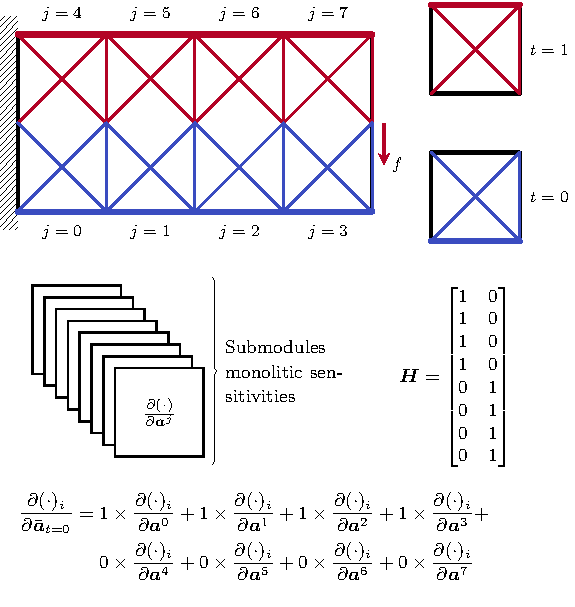
\includegraphics{figures/05_cellular_opt/00_modules_VL_grad/modules_grad.pdf}
    \caption{Notations used for the evaluation of the sensitivities for the modular structure optimization based on the variable linking scheme.}
    \label{fig:05_VL_grad}
\end{figure*}

\section{Numerical application} \label{sec:05_02}
In this section, we formulate multiple test cases used to explore the limits and the characteristics of modular structures and the proposed modular structure optimization formulation \eqrefnotext{eq:05_optim_complete_modular}.

The test cases are optimized using the two-step resolution strategy implemented with five calls of reinitialization (2S-5R) with $n_{\text{max}}=5$. The reinitialization magnitude parameter $\vect{\phi}$ is set up using the same parameters listed in \tabref{tab:05_param}, that leads to $\vect{\phi} = \left[ 0.8000, 0.6400, 0.4096, 0.1677, 0.0281 \right]$.
\begin{margintable}
        \small
    \centering
    \begin{tabular}{cc}
    \toprule
    \textbf{Parameter} & \textbf{Value} \\ \midrule
    $\phi_0$              & 0.8 \\
    $\beta$             & 2 \\
    \bottomrule
    \end{tabular}
    \caption{Reminder of the parameters used to set the reinitialization parameters for the modular optimization. The full list of values and tolerances used for the setup of the optimization algorithm can be found in \tabref{tab:04_param}.}
    \label{tab:05_param}
\end{margintable}

The optimizations are performed using the Python package CVXPY 1.2.2 \sidecite{diamond_cvxpy_2016} with the ECOS 2.0.7 \sidecite{domahidi_ecos_2013} solver to solve the relaxed \gls{lp} Problem \eqrefnotext{eq:05_optim_no_constr_modular}. The \gls{nlp} Problem \eqrefnotext{eq:05_optim_complete_modular} is solved using cyipopt \sidecite{Moore_Mechmotum}, a Python wrapper for IPOPT 3.14.11 \sidecite{wachter_implementation_2006}, a large-scale nonlinear optimization package using PARDISO 6.0 \sidecite{alappat_recursive_2020} as linear solver. 

\subsection{On the equivalence of multi-load cases and modular structures}
\begin{margintable}
    \small
    \centering
    \begin{tabular}{cc}
    \toprule
    \textbf{Parameter}        & \textbf{Value} \\ \midrule
    $L$              & 100     \\
    $E$              & 1     \\
    $\sigma_\text{c}, \sigma_\text{t}$ & $\pm 1$\\
    $P$              & 1   \\
    \bottomrule
    \end{tabular}
    \caption{Material data used for the modular bridge section 2D structure.}
    \label{tab:05_modular_data}
\end{margintable}
The first test case we deal with is a two-dimensional bridge structure segment composed of two subdomains ($n_{\text{sub}} = 2$) with symmetric boundary conditions, as illustrated in \figref{fig:05_cell_multi_eq_bcs}a. In this test case, two vertical loads of magnitude P=1 are applied to the lower side of the design space. The material and geometrical details are given in \tabref{tab:05_modular_data} and are normalized and adimensional for simplicity. Each subdomain of the structure is discretized using a 15x15 fully connected ground structure, with a number of candidates $\bar{n}=25200$ per subdomain. It is important to note that, for this example, buckling constraints have been deactivated.

Additionally, a similar structure is optimized, comprising only a single subdomain, subjected to two distinct load cases, denoted as $P_1$ and $P_2$. These loads are positioned at precisely the same distance from the support as the structure with multiple subdomains, as illustrated in \figref{fig:05_cell_multi_eq_bcs}b. The subdomain is discretized using the same 15x15 fully connected ground structure.

\begin{figure}[]
    \hspace*{\fill}
    \subcaptionbox{}{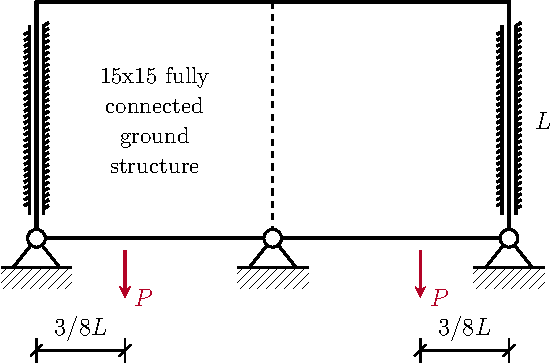
\includegraphics[height=4.15cm]{figures/05_cellular_opt/00_cell_multi_eq_bcs/cell_bcs.pdf}}
    \hfill
    \subcaptionbox{}{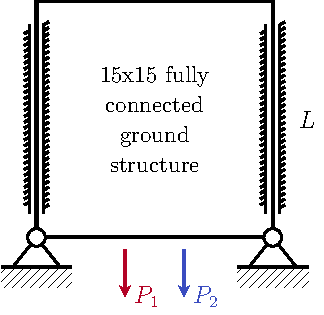
\includegraphics[height=4.15cm]{figures/05_cellular_opt/00_cell_multi_eq_bcs/multiload_bcs.pdf}}
    \hspace*{\fill}
    \caption{Boundary conditions of the multi-subdomains (a) and the multi-load cases (b) test cases.}
    \label{fig:05_cell_multi_eq_bcs}
\end{figure}

\begin{table}
    \centering
    \small
    \begin{tabular}{lcc}
        \toprule
        \textbf{Quantity} & Multi-subdomain & Multi-loads \\ \midrule
    $N_\text{sub}$       &2& 1   \\
    $N_\text{opt}\;(N_\text{el})$ & 62 (50400)&31 (25200)  \\
    $V$ &  182.692 & 91.346 \\ \bottomrule
    \end{tabular}
    \caption{}
    \label{tab:05_}
    \end{table}

The optimization is carried out for both structures, utilizing the material data specified in \tabref{tab:05_modular_data}. The joint cost is set at $s = 0.05$ for the multi-subdomain structure and $s = 0.1$ for the multi-load case structure. the graphical representation of the optimized structures is given in \figref{fig:05_cell_multi_eq}. Remarkably, the resulting subdomain topologies are identical, with the volume of the multi-subdomain structure $V_1$ being precisely twice the volume of the multi-load cases structure $V_2$. 

This straightforward example highlights an interesting aspect of modular structure optimization that aligns with common sense. When a loaded structure is divided into multiple subdomains, each subdomain, when isolated and subjected to appropriate boundary conditions defined by the reaction forces of adjacent bars and supports, experiences multiple loading conditions. By imposing modularity constraints on all these subdomains, the optimization process seeks the optimal structure that simultaneously meets the mechanical needs of all these diverse load cases. Hence, there exists an equivalence between optimizing a multi-subdomain structure with modular constraints and performing a multi-load case optimization solely on the module. Moreover, these examples confirm the necessity of adding kinematic compatibility constraints when addressing modularity constraints.
\begin{figure}[]
    \hspace*{\fill}
    \subcaptionbox{}{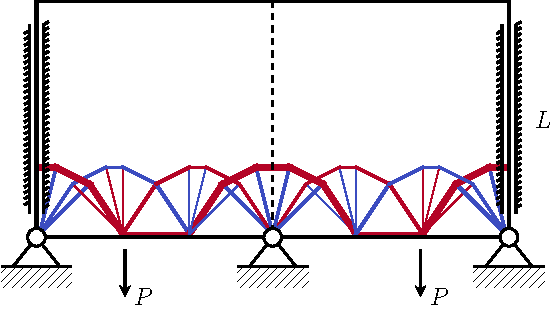
\includegraphics[height=3.5cm]{figures/05_cellular_opt/00_cell_multi_equivalence/cell.pdf}}
    \hfill
    \subcaptionbox{}{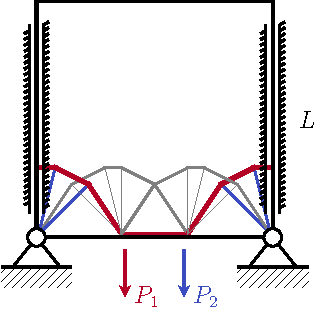
\includegraphics[height=3.5cm]{figures/05_cellular_opt/00_cell_multi_equivalence/multiload.pdf}}
    \hspace*{\fill}
    \caption{Optimized structures of the multi-subdomains (a) and the multi-load cases (b) test cases. The resulting module topology is equal for the two cases. In red the bars are in a tensile state, and in blue the bars are in a compressive state.}
    \label{fig:05_cell_multi_eq}
\end{figure}

\subsection{Parametric study on the number of subdomains and the complexity of the module}
\begin{marginfigure}
    \centering
    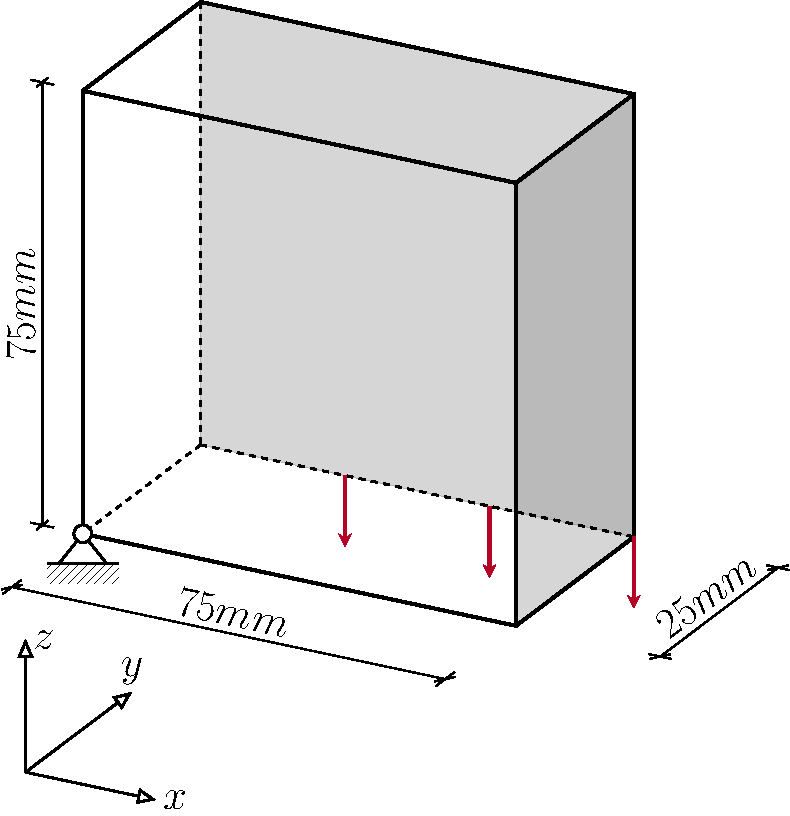
\includegraphics[width=\linewidth]{figures/05_cellular_opt/00_supported_bc/supported_3D_symm.pdf}
    \caption{Symmetric boundary conditions of the simply supported 3D beam. In gray are the symmetry planes of the test case.}
    \label{fig:05_symm_support_bc}
\end{marginfigure}
\begin{margintable}
    \small
    \centering
    \begin{tabular}{cc}
    \toprule
    \textbf{Parameter}        & \textbf{Value} \\ \midrule
    $E$              & \qty{2.7}{GPa}     \\
    $\nu$            & 0.3   \\
    $\sigma_\text{c}, \sigma_\text{t}$ & $\pm $\qty{55}{MPa} \\
    $\rho$              & \qty{1.14}{\gram\per\cubic\centi\metre}   \\
    $P$              & \qty{100}{N}   \\
    \bottomrule
    \end{tabular}
    \caption{Material data used for the simply supported 3D beam optimization.}
    \label{tab:05_3D_supp_mat}
\end{margintable}
\begin{marginfigure}
    \centering
    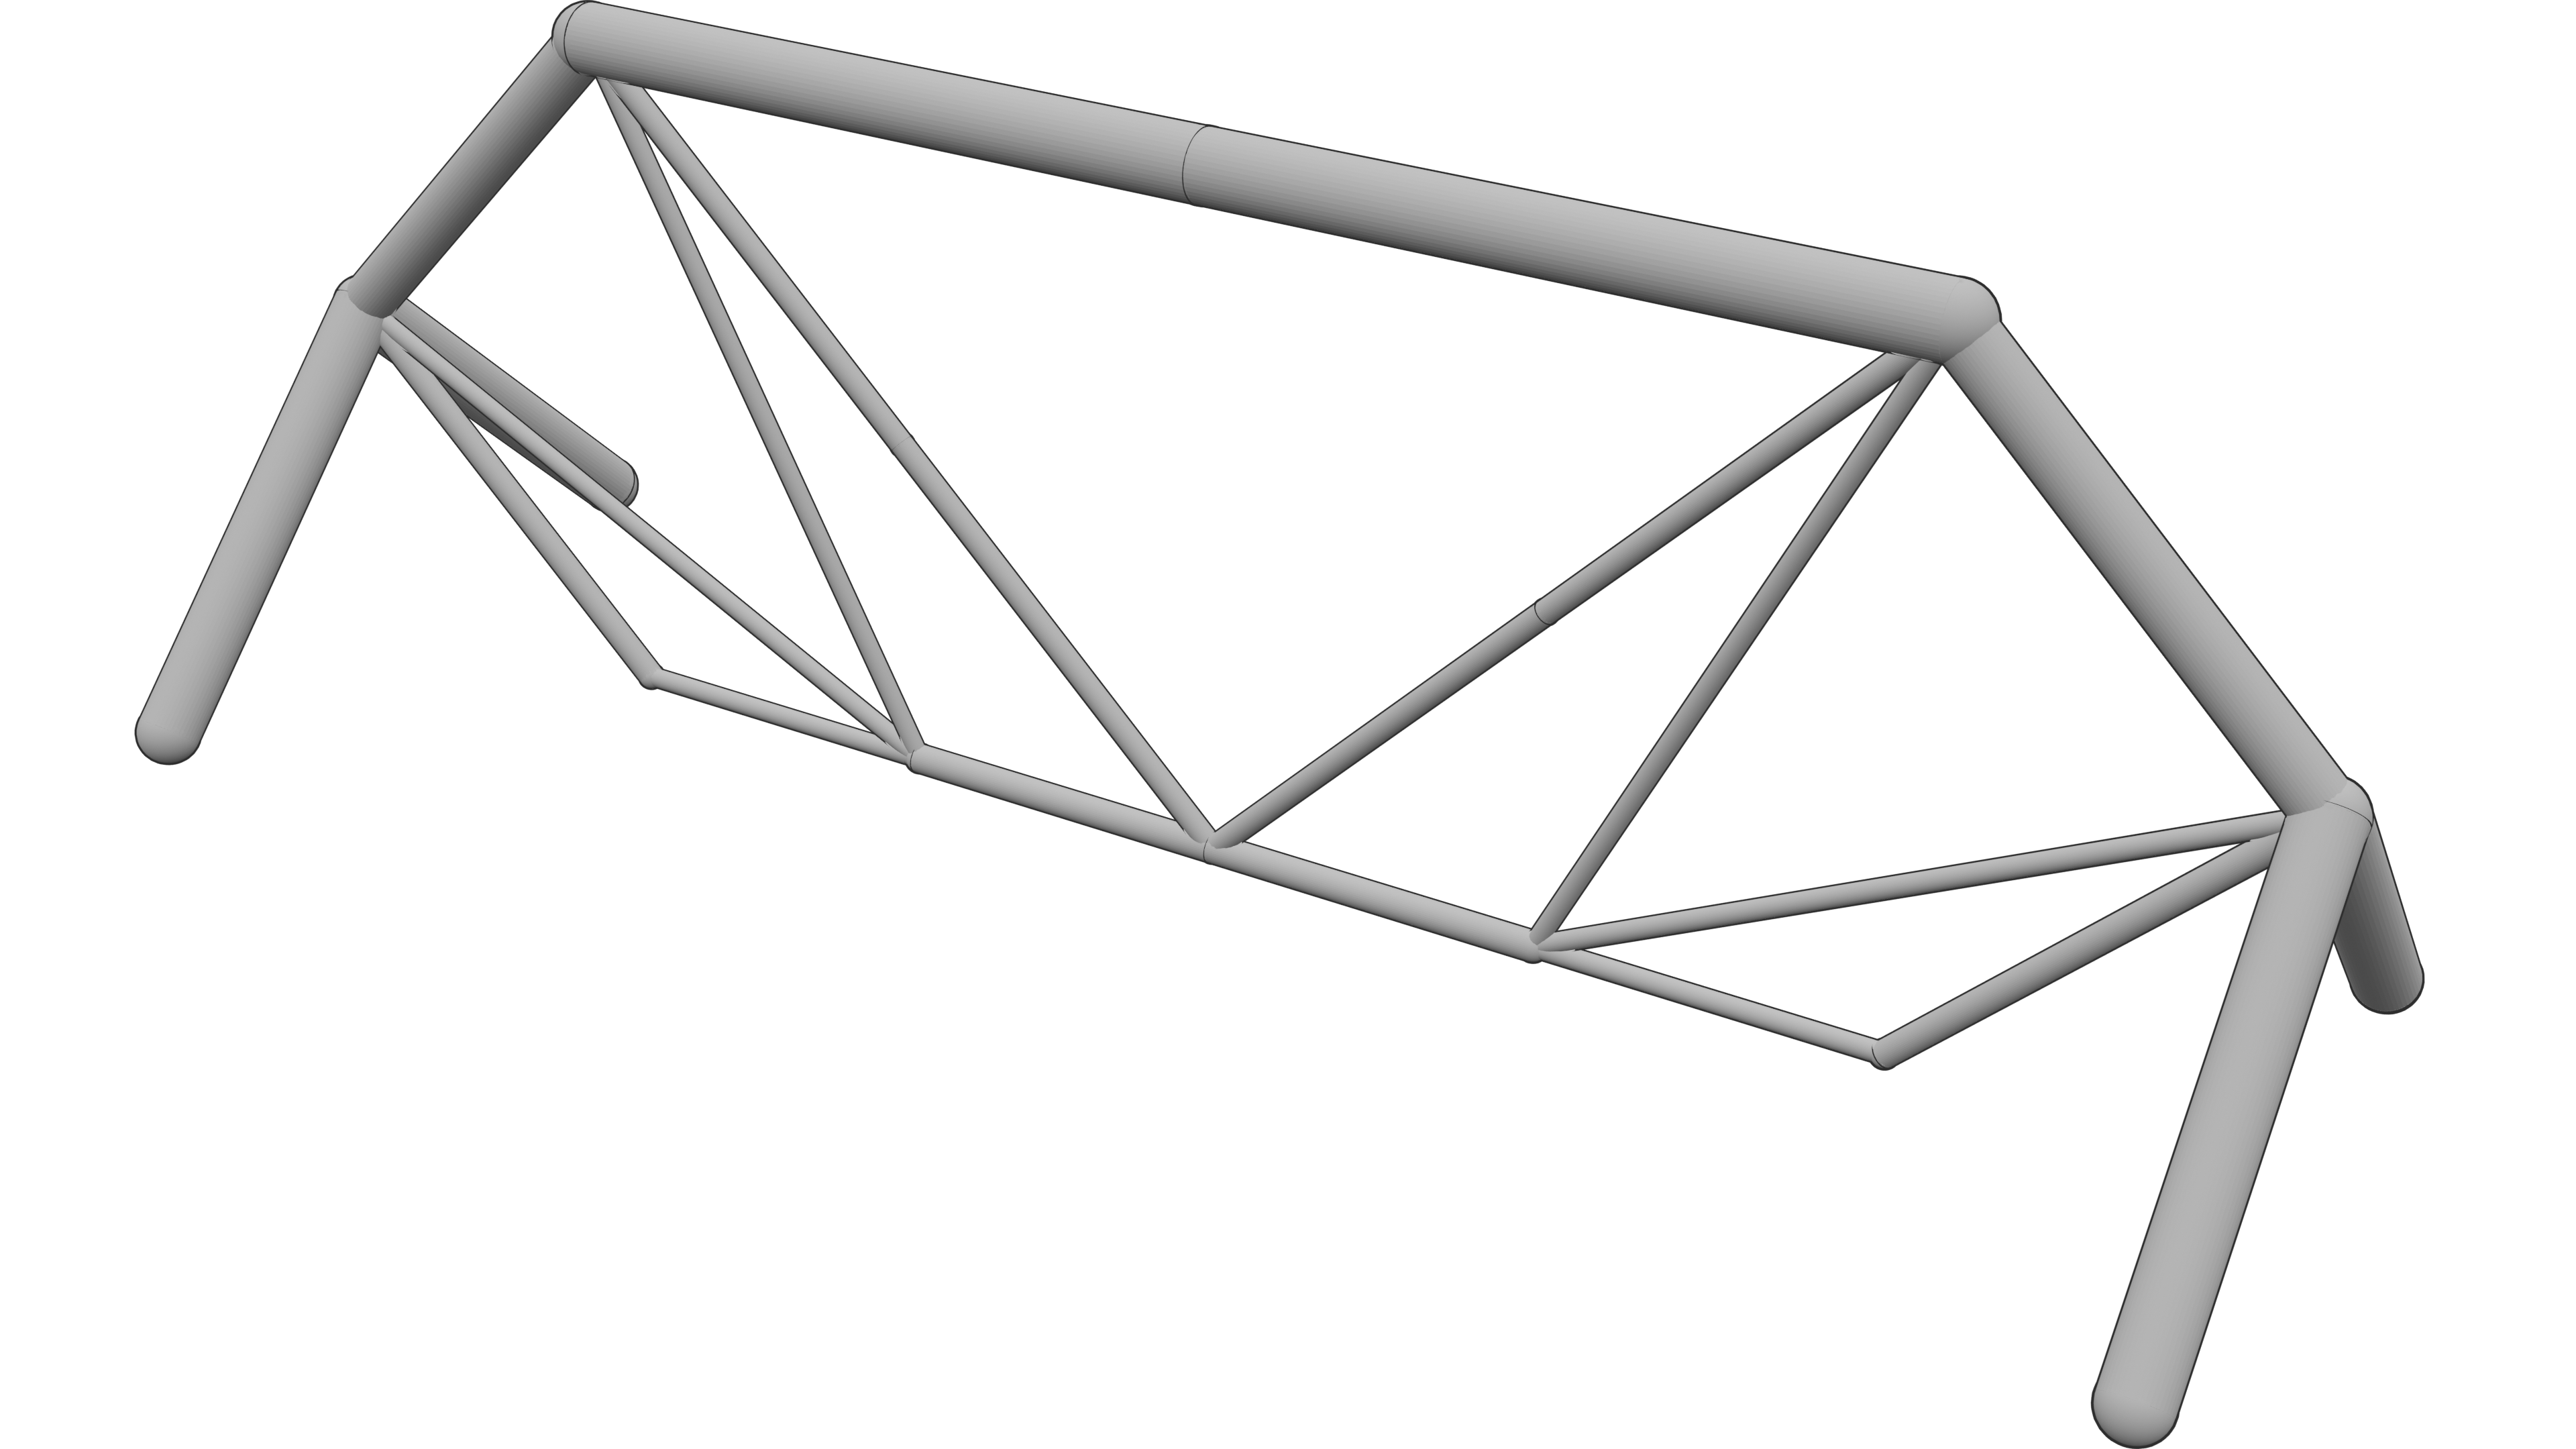
\includegraphics[width=\linewidth]{figures/04_TTO_improvements/16_supported_3D_sol/04_Topology_NLP_iso-min.png}
    \caption{Perspective view of the monolithic simply supported 3D beam optimized structure with $V=\qty{9.907}{\centi\meter^3}$}
    \label{fig:05}
\end{marginfigure}
Here, we perform a parametric study on the modular parameters that we use to optimize the simply supported 3D truss, which was previously analyzed as a monolithic structure in \secref{sec:04_simply_supp}. In this study, we focus on a single module $N_\text{T} = 1$, excluding for the moment an examination of the impact of multiple module topologies on the optimized structure. Additionally, we restrict our investigation to a cubic cell shape. A summary of the loading case, as well as the geometric and material properties of the test case, is presented in \tabref{tab:05_3D_supp_mat} and depicted in \figref{fig:05_symm_support_bc}.

We introduce two new metrics used to enhance our understanding of how modular structures are subjected to loading. The first metric, named the structural efficiency index and denoted as $\varphi$, enables a rapid assessment of how close the structure is to the optimal fully stressed state as described by Michell \sidecite{michell_limits_1904}. Since we are accounting for not only tensile and compressive stress but also local buckling, we define a bar as fully stressed when it activates one or more of the three mechanical failure constraints. It is defined by the equation:
\begin{equation}
    \varphi = \frac{N_\text{opt,f}\times100}{N_\text{opt}}.
\end{equation}
Here, $N_\text{opt,f}$ represents the number of bars that activate either the tensile stress, compressive stress, or buckling constraints and is expressed as:
\begin{equation}
    N_\text{opt,f} = \operatorname{card}(\{i\;|\;c_\text{f,i} > 0.95\}),
\end{equation}
where $\vect{c}_\text{f}=\max{\left(-\vect{q} /\sigma_c \vect{a},\:\vect{q} /\sigma_t \vect{a},\:\vect{q}/\vect{q}_{\text{crit}}\right)}$ represent the normalized mechanical failure criterion and $\operatorname{card}(\{\cdot\})$ represent the cardinality of the set $\{\cdot\}$.

The second metric, denoted as $\psi$, is defined as the mean value of the normalized mechanical failure criterion $\vect{c}_\text{f}$, weighted by the volumes of individual bars $\vect{v}$:
\begin{equation}
    \psi = \frac{1}{V} \left( \sum_{i=0}^{N_\text{opt}} v_i c_{\text{f},i} \right)
\end{equation}
This parameter ranges between 0 and 1, with higher values indicating that, on average, bars are closer to the upper limit of one of the mechanical failure constraints. Notably, greater importance is attributed to more voluminous bars.

\paragraph{Influence of the number of the subdomains}
We begin by examining the impact of the number (and consequently, the scale, interchangeably used here) of subdomains $N_\text{sub}$ in the structure. The structure is partitioned into varying numbers of cubic and equal-sized subdomains while keeping the test case and material constant. Specifically, the entire structure is subdivided into 6x2x3, 12x4x6, 18x6x9, and 30x10x15 submodules along the $X$, $Y$, and $Z$ axes, and each subdomain is discretized by a 2x2x2 fully connected ground structure with $n_{\text{bar}} = 28$. The same analysis is also conducted on a 3x3x3 fully connected ground structure with $n_{\text{bar}} = 351$ to ensure that trends remain consistent across varying cell complexities.

\begin{marginfigure}
    \centering
    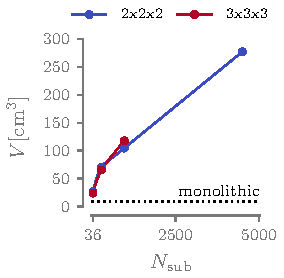
\includegraphics{figures/05_cellular_opt/00_module_scale_tab/scale_tab_v.pdf}
    \caption{Influence of the number of subdomains on the volume of the optimized modular structure.}
    \label{fig:05_scale_v}
\end{marginfigure}

\begin{marginfigure}
    \centering
    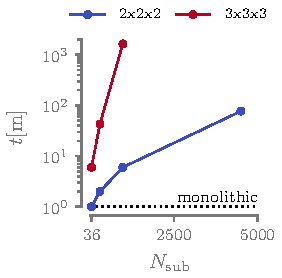
\includegraphics{figures/05_cellular_opt/00_module_scale_tab/scale_tab_t.pdf}
    \caption{Influence of the number of subdomains on the computational time of the optimization.}
    \label{fig:05_scale_t}
\end{marginfigure}

The parametric findings on the impact of the number of subdomains in the structure are summarized in \tabref{tab:05_scale_results}. The table presents numerical results alongside graphical representations of the optimized structures' modules for varying sizes of the repeating module. The first key observation is the significant influence of the module scale on the optimized volume. This relationship is evident in \figref{fig:05_scale_v}, where the volume exhibits an almost linear correlation with the number of submodules, a trend that persists even for the higher complexity 3x3x3 modules. Regarding computational time, a similar relationship is noted. Despite the number of design variables remaining constant, the increase is attributed to the growing number of mechanical constraints. It is important to highlight that in modular optimization, mechanical constraints are evaluated for every member of the structure, not just within the module. Finally, the number of active bars in the optimized module shows little dependence on the module scale.

A graphical representation of the 3D structures is provided in \figref{fig:05_scale_results}, showing isometric views as well as views on the XZ planes for the case with a module featuring a 2x2x2 ground structure. It is interesting to observe how, with increasing physical dimensions of the module, the optimizer naturally converges toward solutions that prioritize long tensile members and short compressive members to satisfy local buckling constraints. However, as the module size decreases (as seen in the 30x10x15 results), and consequently, the buckling effective length of the members diminishes the optimized design transitions to a configuration where both tensile and compressive members are present. This observation aligns with the findings of Sigmund on Michell-like structures \sidecite{sigmund_non-optimality_2016}.

\begin{table*}
    \centering
    \small
    \begin{tabular}{lx{1.4cm}x{1.4cm}x{1.4cm}x{1.4cm}x{1.45cm}x{1.4cm}x{1.4cm}x{1.4cm}x{1.4cm}}
        \toprule
        \multirow{2}{*}{\textbf{Quantity}}         & 7x3x4 &\multicolumn{4}{l}{2x2x2} & \multicolumn{3}{l}{3x3x3} \\ 
             \cmidrule(lr){2-2} \cmidrule(lr){3-6} \cmidrule(lr){7-9} 
     &1x1x1& 6x2x3      & 12x4x6     &  18x6x9    &  30x10x15\textsuperscript{\emph{a}}   &   6x2x3      & 12x4x6     &  18x6x9      \\
     & -- & 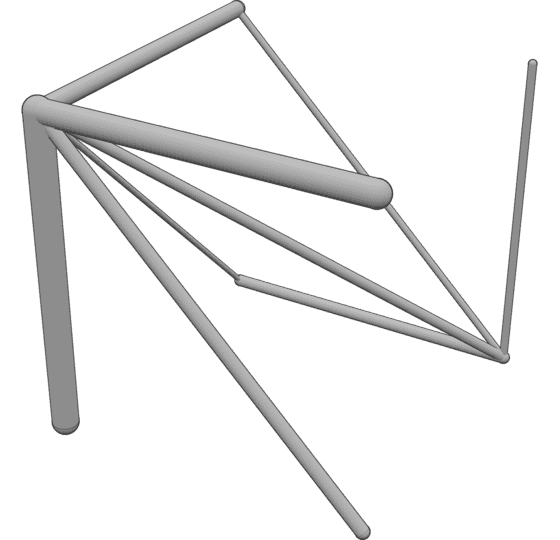
\includegraphics[width=1.3cm]{figures/05_cellular_opt/00_module_scale_cell/6x2x3_2x2x2_c.png}    &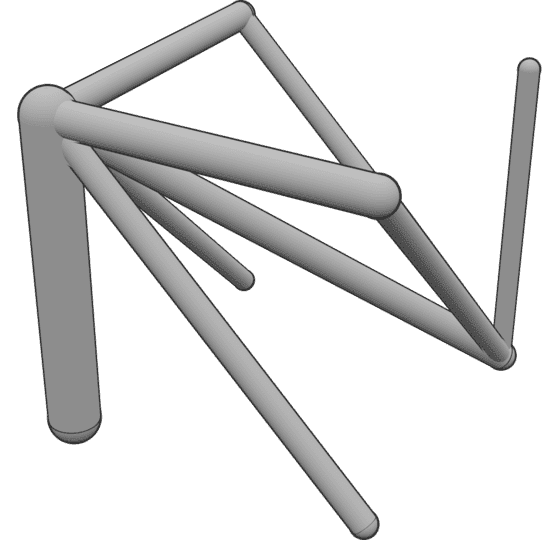
\includegraphics[width=1.3cm]{figures/05_cellular_opt/00_module_scale_cell/12x4x6_2x2x2_c.png}&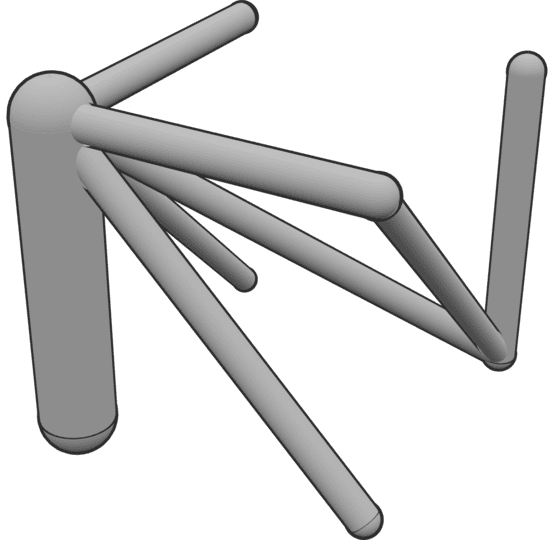
\includegraphics[width=1.3cm]{figures/05_cellular_opt/00_module_scale_cell/18x6x9-2x2x2_c.png}&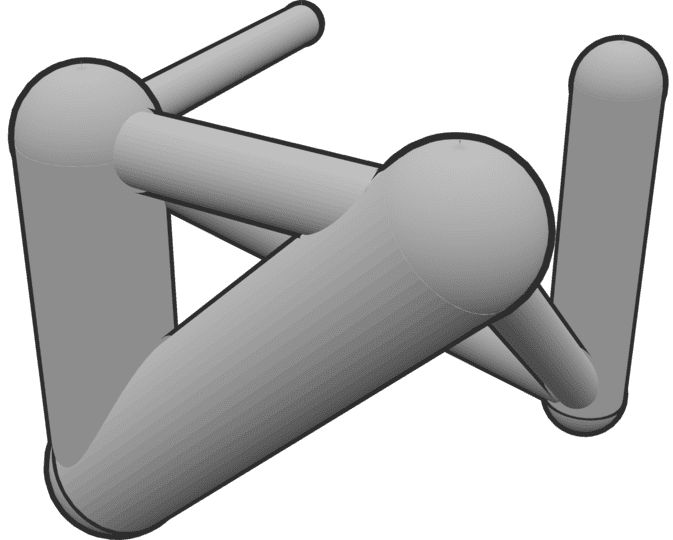
\includegraphics[width=1.3cm]{figures/05_cellular_opt/00_module_scale_cell/30x10x15-2x2x2_c.png}&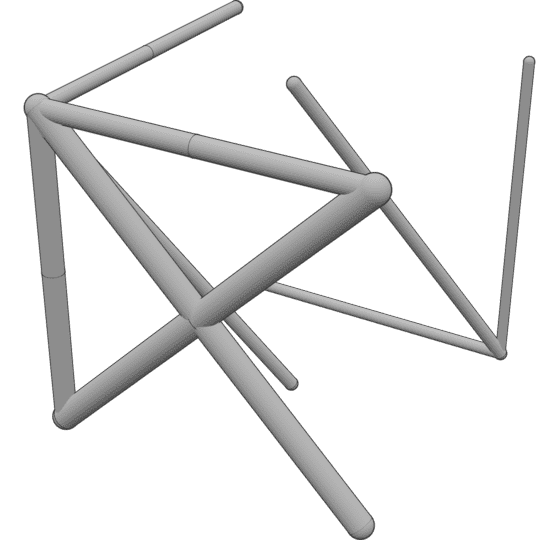
\includegraphics[width=1.3cm]{figures/05_cellular_opt/00_module_scale_cell/6x2x3_3x3x3_c.png}&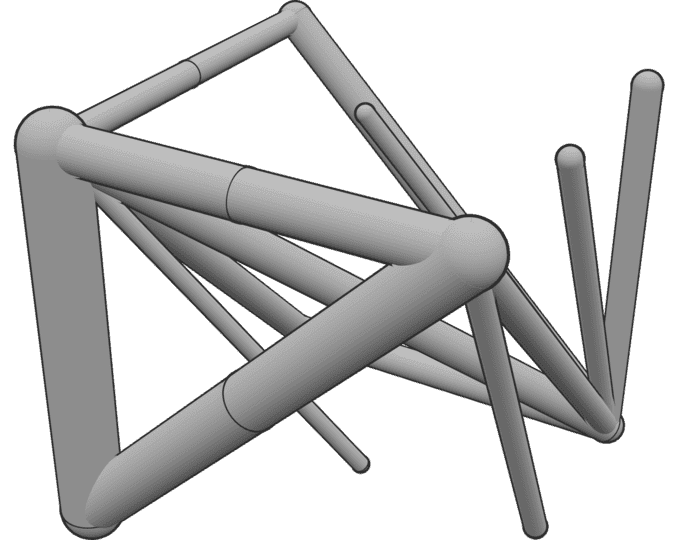
\includegraphics[width=1.3cm]{figures/05_cellular_opt/00_module_scale_cell/12x4x6_3x3x3_c.png}&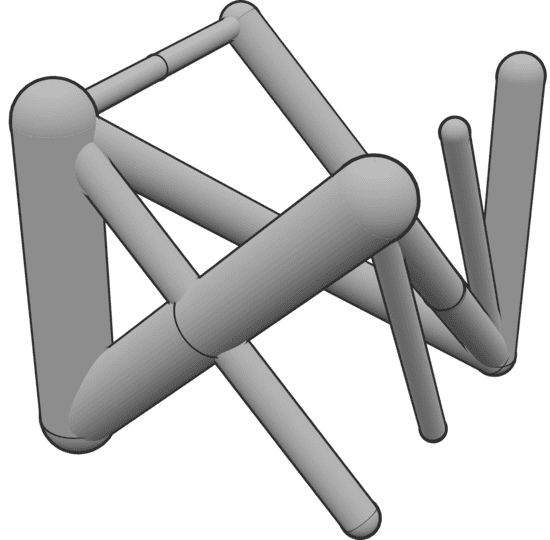
\includegraphics[width=1.3cm]{figures/05_cellular_opt/00_module_scale_cell/18x6x9-3x3x3_c.png}        \\
    $\bar{n}_\text{opt}\;(\bar{n})$ &1984&9 (28)&9 (28) &8 (28)&8 (28)&19 (351)&15 (351)& 16 (351)\\
    $N_\text{sub}$         &1&36&288&972&4500&36&288&972  \\
    $N_\text{opt}\;(N_\text{el})$ &20 (1984)&324 (1008)&2592 (8064)&7776 (27216)&36000 (126000)&468 (12636)&4320 (101088)&  15552 (341172)       \\
    $V$ [\unit{cm^3}]&9.907&27.074&70.559&104.891&277.238&24.323&65.723&117.904         \\
    $V$ [\unit{\percent}] &1.761&4.812&12.544&18.648&49.288&4.324&11.684&20.960         \\
    C [\unit{J}]    &3.71&4.22&3.35&3.19&1.12&3.63&1.84&2.02\\
    $a_\text{max}$ [\unit{mm^2}]   &37.61&9.40&5.45&5.45&3.55&5.33&2.60&3.14         \\
    $\varphi$   &\qty{100.00}{\percent}&\qty{14.81}{\percent}&\qty{1.85}{\percent}&\qty{0.67}{\percent}&\qty{0.12}{\percent}&\qty{20.51}{\percent}&\qty{1.46}{\percent}&\qty{0.62}{\percent}         \\
    $\psi$   &1.000&0.446&0.178&0.105&0.030&0.327&0.127&0.096\\
    t     &\hms{0;0;4}&\hms{0;0;6}&\hms{0;0;48}&\hms{0;5;6}&\hms{1;17;00}&\hms{0;5;42}&\hms{0;42;50}& \hms{27;17;00} \\ \bottomrule
    \end{tabular}
    \\
    \scriptsize{\textsuperscript{\emph{a}}In this test case the minimum slenderness limit is relaxed to $\lambda_\text{max}=10$ instead of 15.}
    \caption{Numeric results of the parametric study on the influence of the number of subdomains on the optimized structures.}
    \label{tab:05_scale_results}
    \end{table*}

    \begin{figure*}
        \hspace*{\fill}
        \subcaptionbox{}{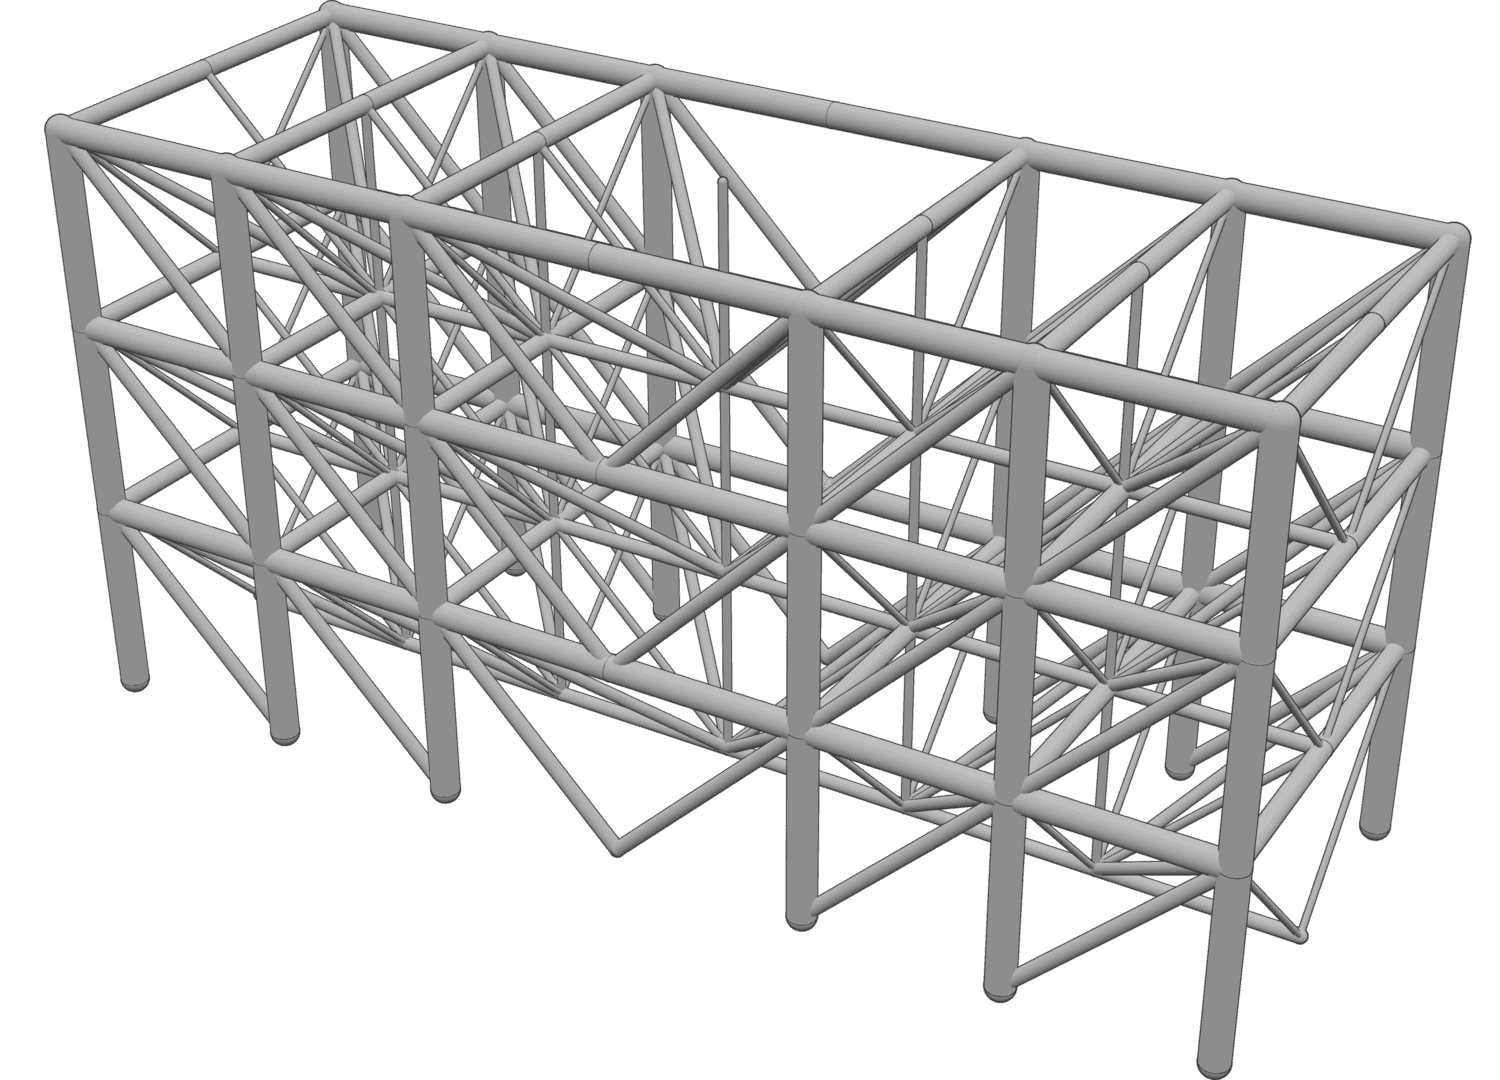
\includegraphics[width=0.23\linewidth]{figures/05_cellular_opt/00_module_scale/6x2x3_2x2x2.png}}
        \hfill
        \subcaptionbox{}{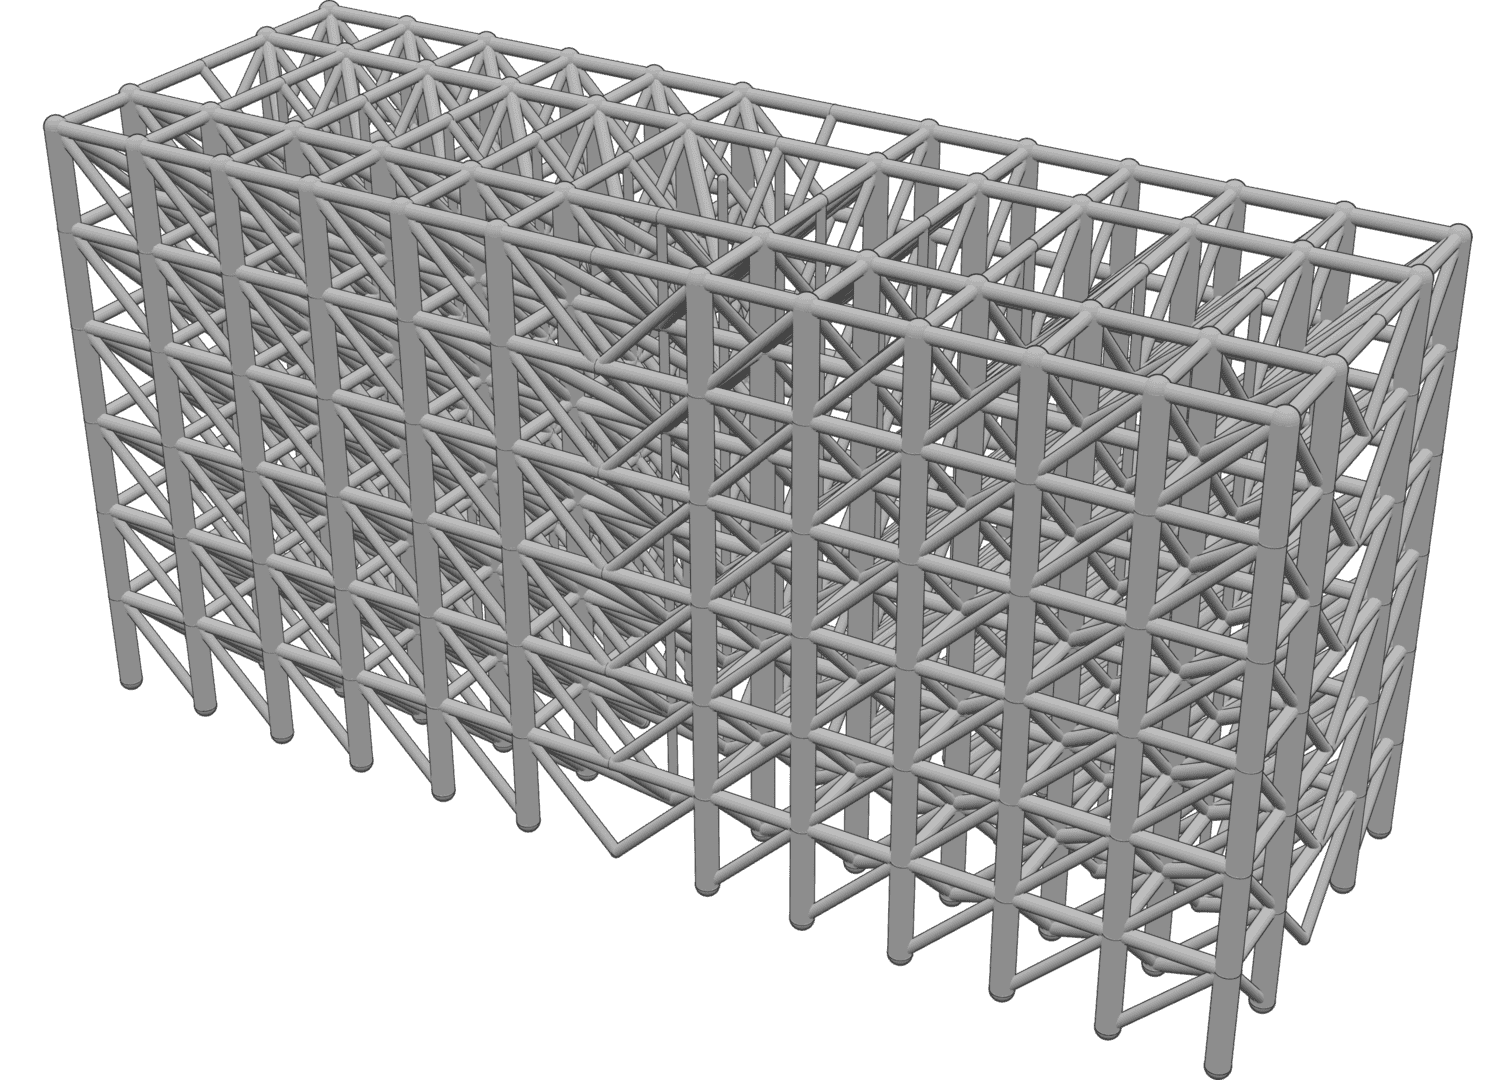
\includegraphics[width=0.23\linewidth]{figures/05_cellular_opt/00_module_scale/12x4x6_2x2x2.png}}
        \hfill
        \subcaptionbox{}{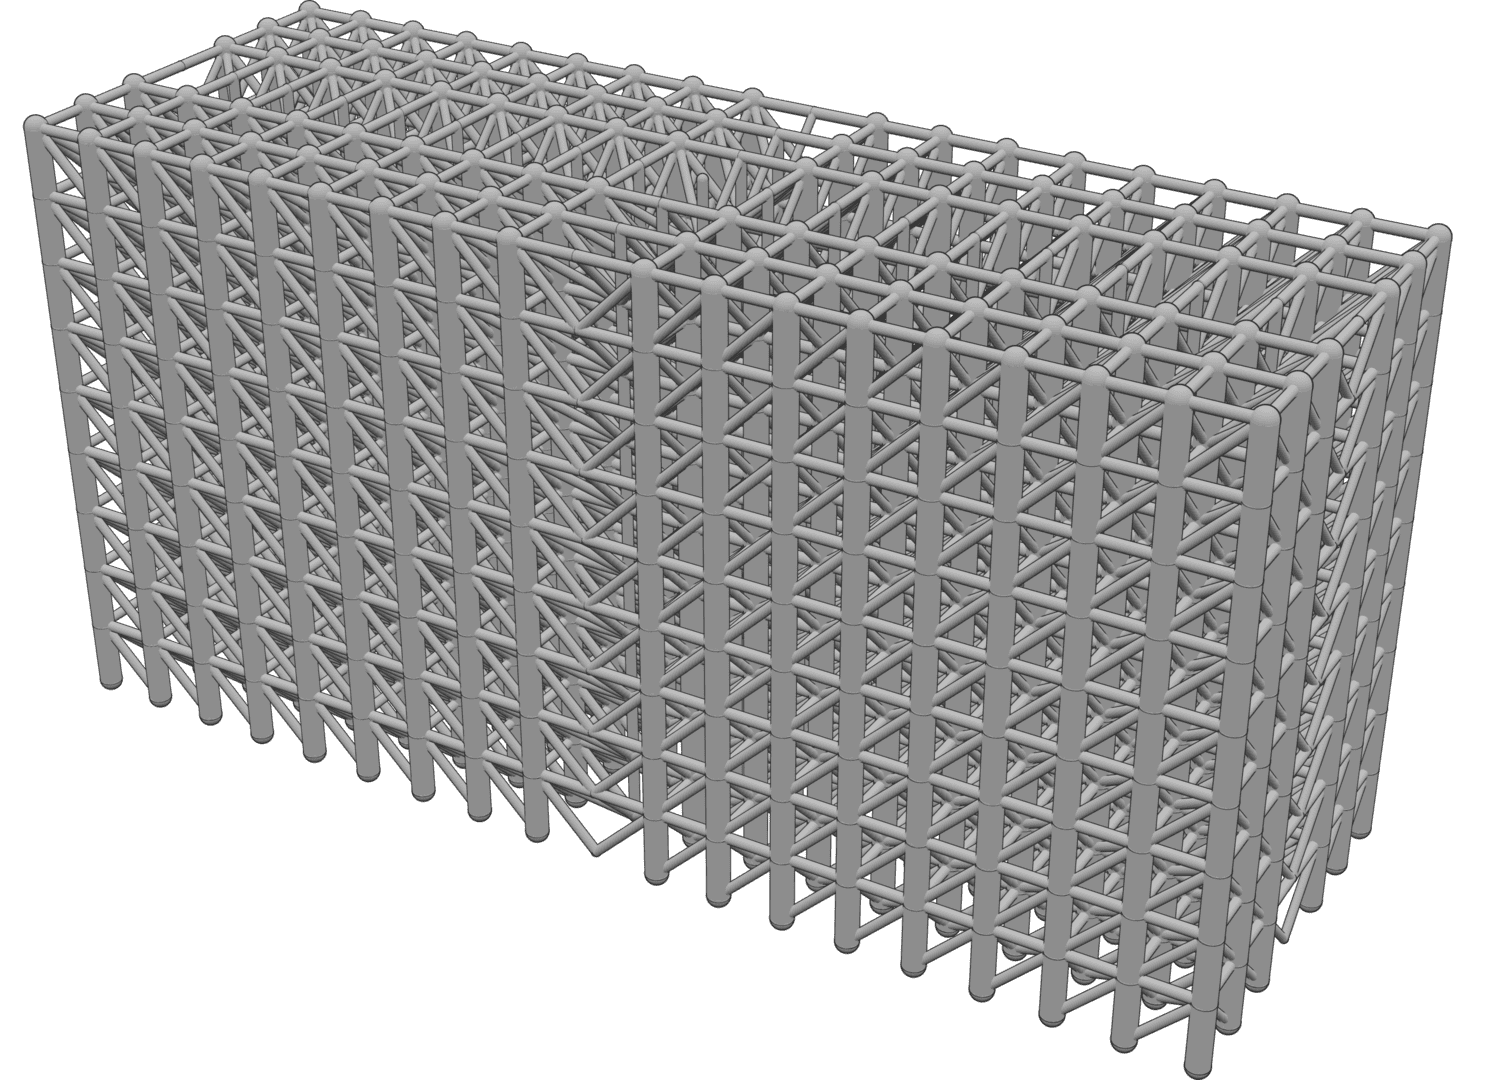
\includegraphics[width=0.23\linewidth]{figures/05_cellular_opt/00_module_scale/18x6x9_2x2x2.png}}
        \hfill
        \subcaptionbox{}{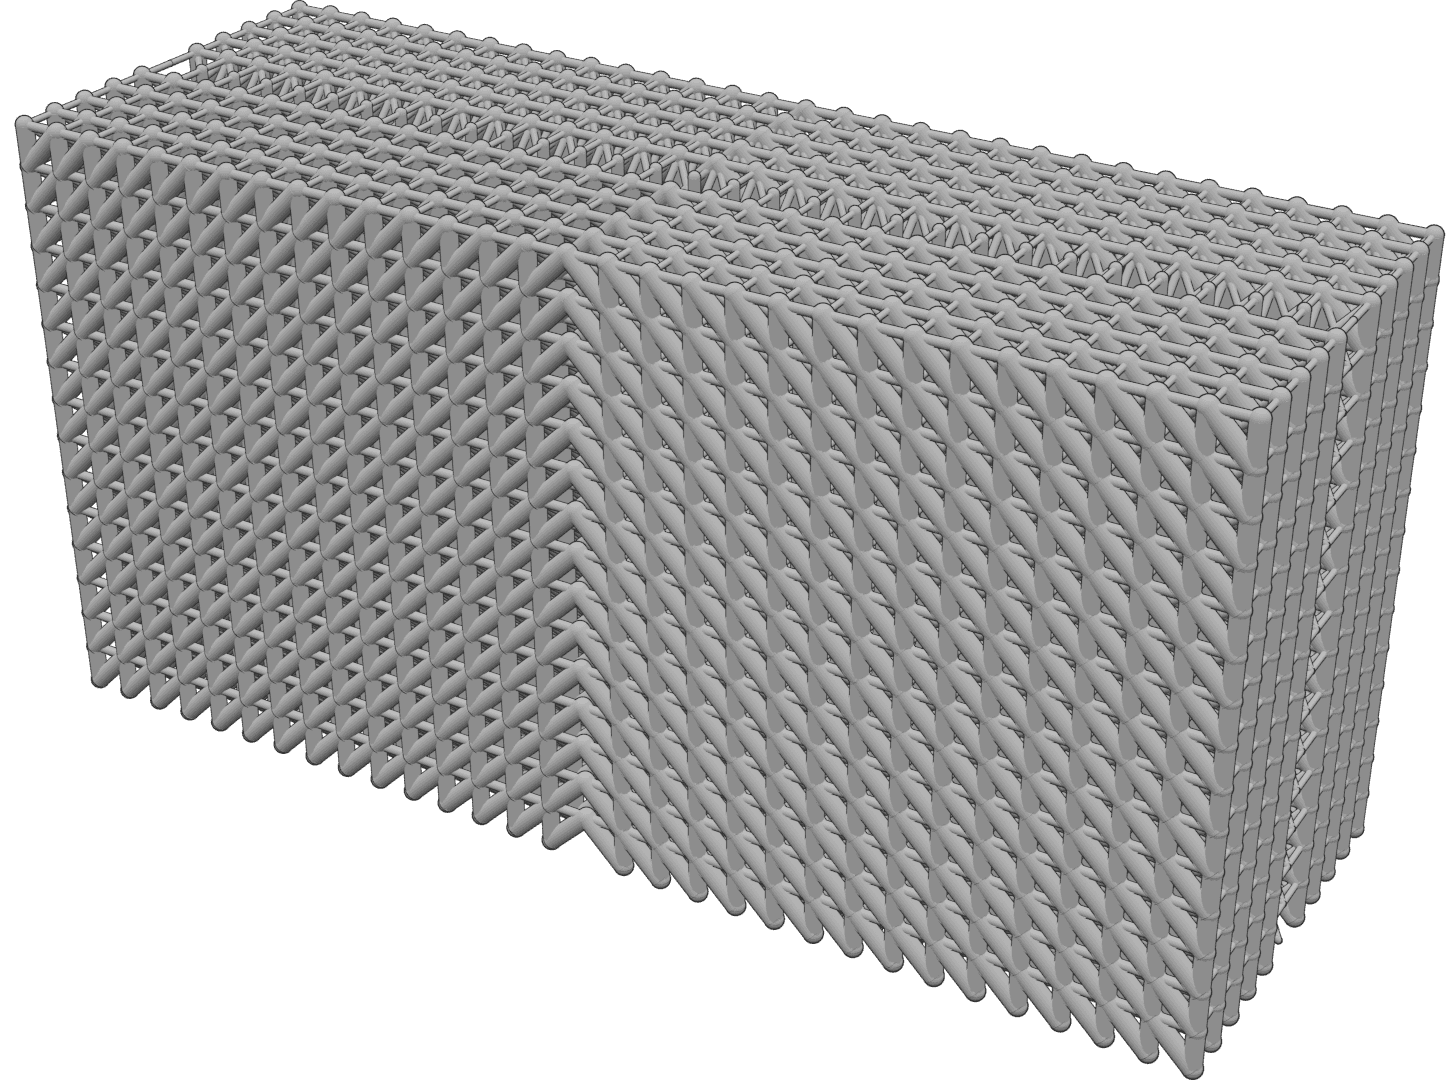
\includegraphics[width=0.23\linewidth]{figures/05_cellular_opt/00_module_scale/30x10x15_2x2x2.png}}
        \hspace*{\fill}
        \bigskip
        \hspace*{\fill}
        \subcaptionbox{}{\includegraphics[width=0.23\linewidth]{figures/05_cellular_opt/00_module_scale/6x2x3_2x2x2_XZ.png}}
        \hfill
        \subcaptionbox{}{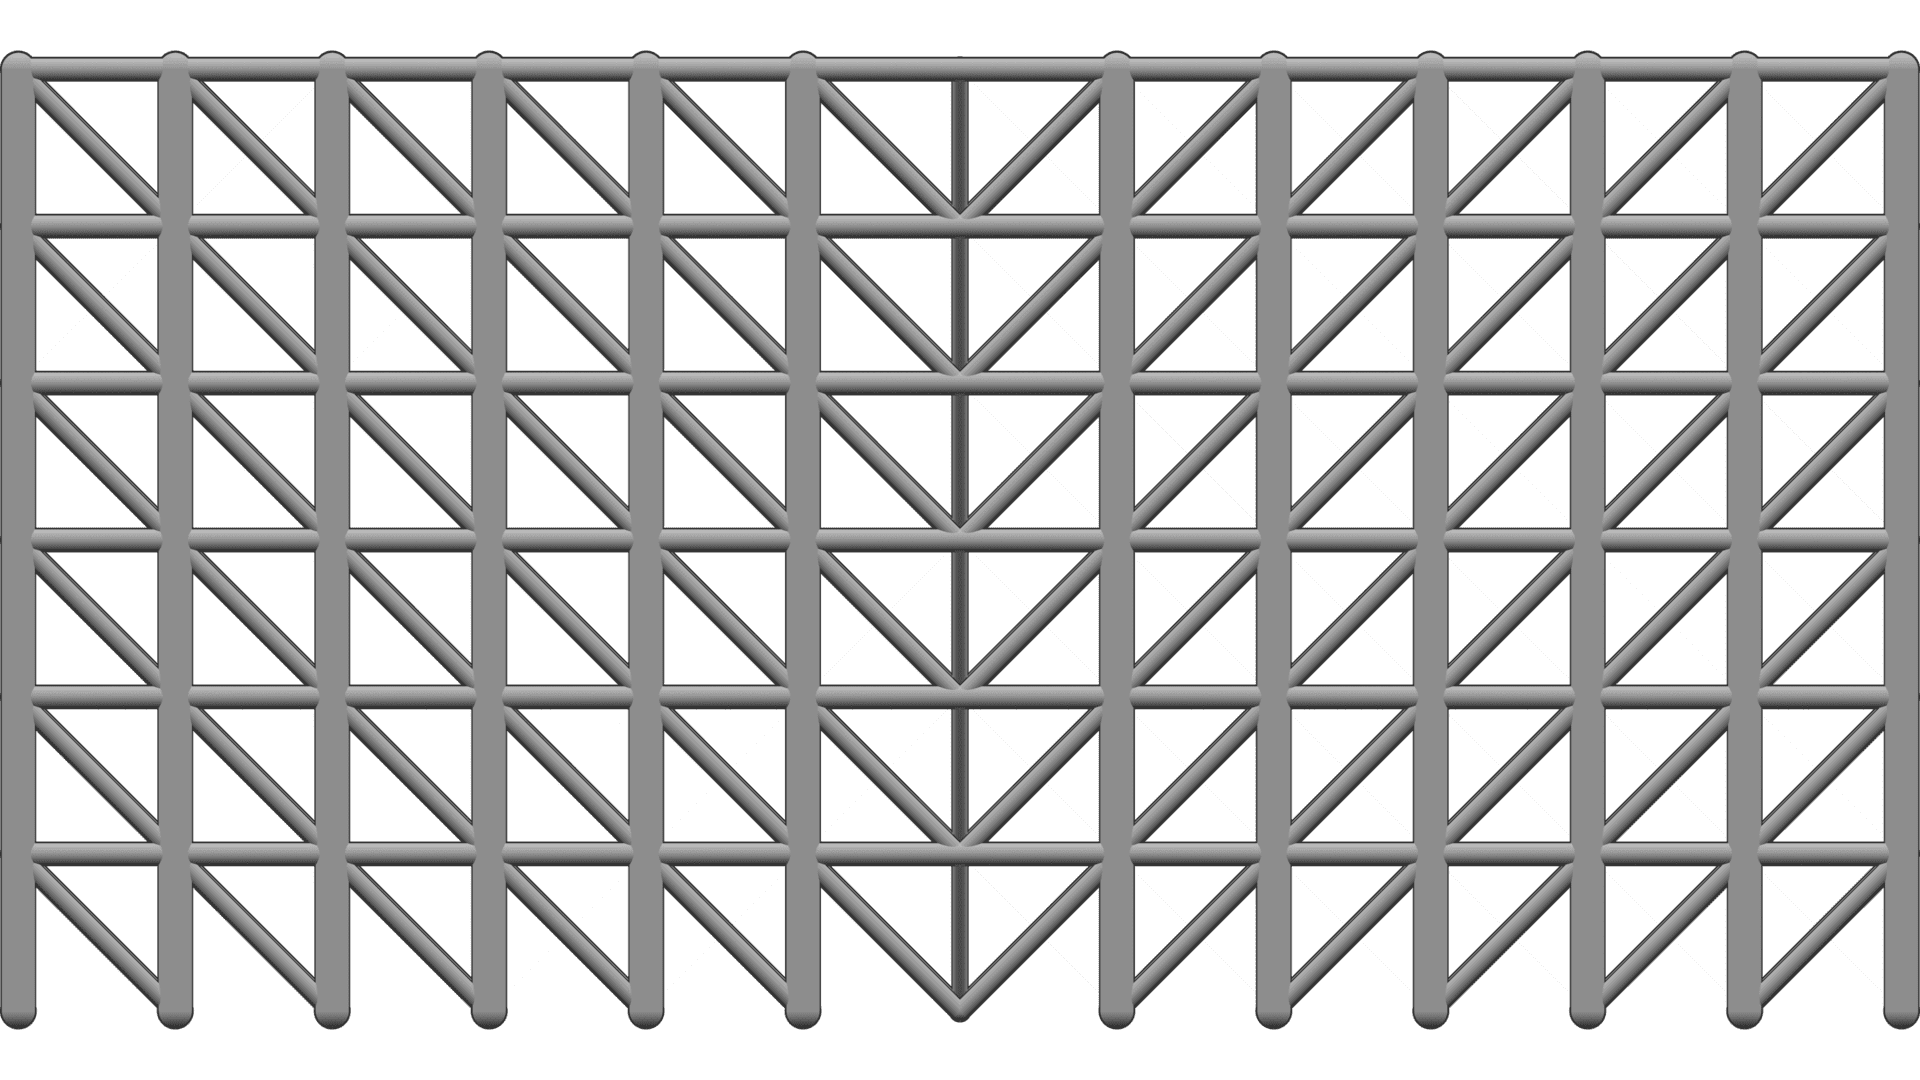
\includegraphics[width=0.23\linewidth]{figures/05_cellular_opt/00_module_scale/12x4x6_2x2x2_XZ.png}}
        \hfill
        \subcaptionbox{}{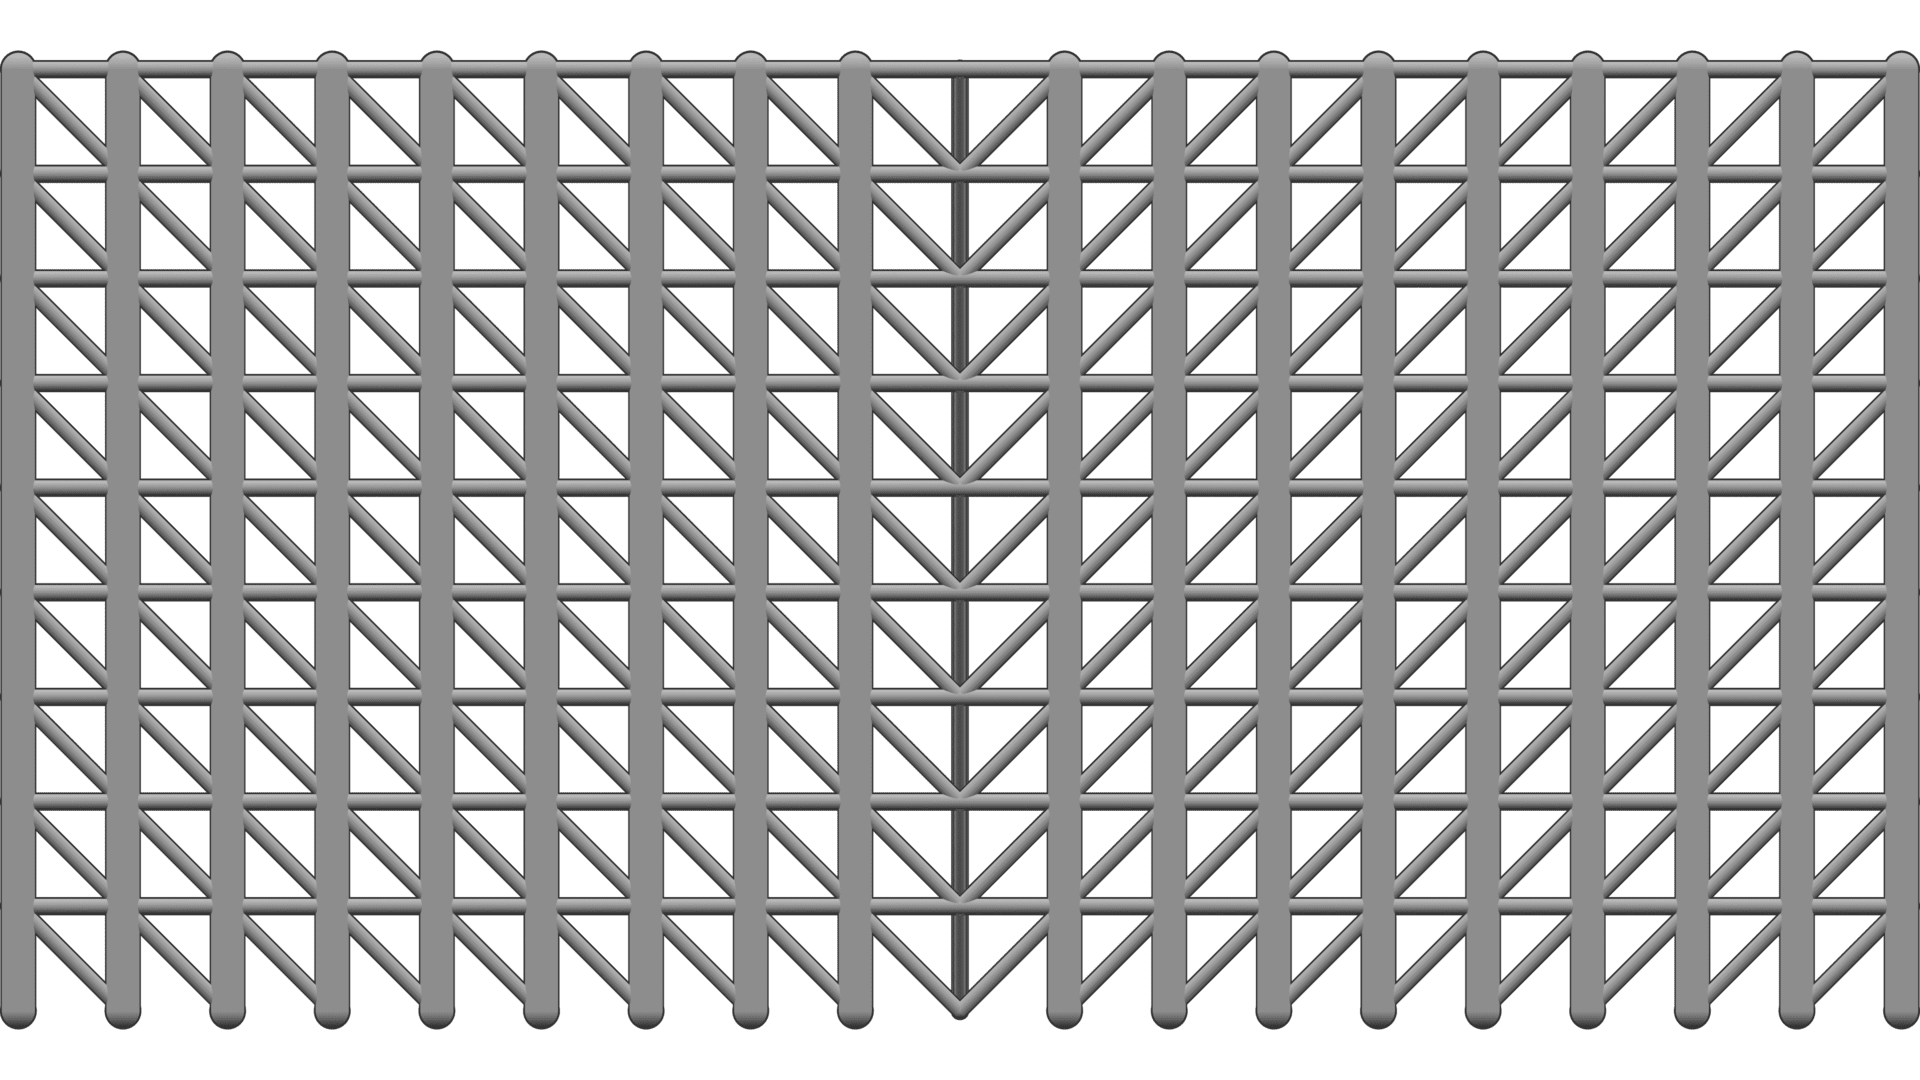
\includegraphics[width=0.23\linewidth]{figures/05_cellular_opt/00_module_scale/18x6x9_2x2x2_XZ.png}}
        \hfill
        \subcaptionbox{}{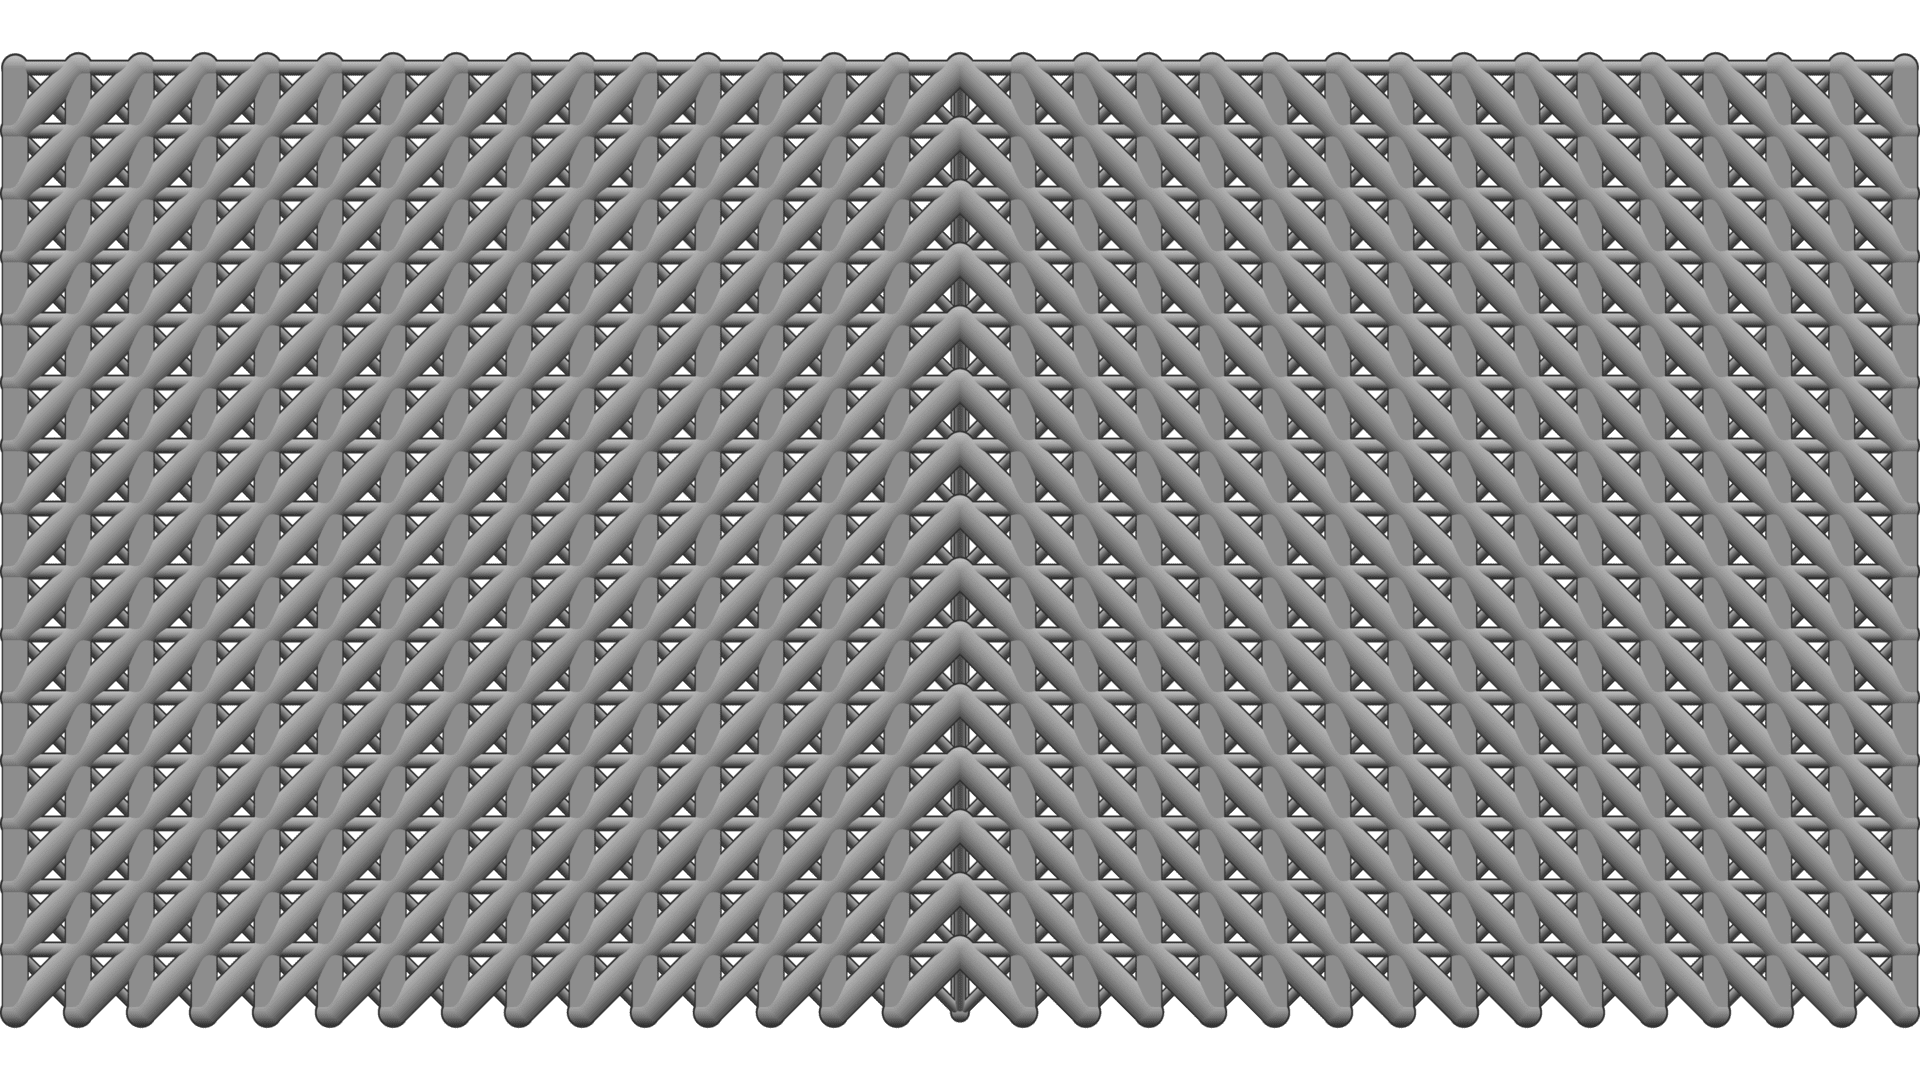
\includegraphics[width=0.23\linewidth]{figures/05_cellular_opt/00_module_scale/30x10x15_2x2x2_XZ.png}}
        \hspace*{\fill}
        \caption{Rendering of the optimized structures with 6x2x3 (a-e), 12x4x6 (b-f), 18x6x9 (c-g), and 30x10x15 (d-h) subomains. The module presents a 2x2x2 complexity.}
        \label{fig:05_scale_results}
    \end{figure*}

    In an attempt to understand why the volume is significantly influenced by the number of submodules, we visualize the trends of the parameters $\varphi$ and $\psi$ in \figref{fig:05_scale_param}. As depicted, every bar in the monolithic structure activates either the buckling or the stress constraint, resulting in $\varphi=100\%$ and $\psi=1$. However, this is not true for any of the modular structures, as seen in the case of 12x4x6-3x3x3, where numerous bars remain inactive and are represented in gray.
    \begin{marginfigure}
        \centering
        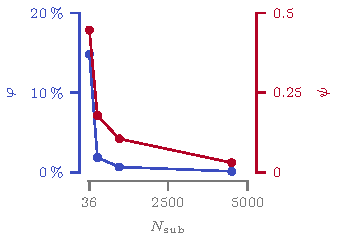
\includegraphics[width=\linewidth]{figures/05_cellular_opt/00_module_scale_tab/scale_tab_param.pdf}
        \caption{Influence of the number of subdomains on the loading metrics $\varphi$ and $\psi$ of the optimized structures.}
        \label{fig:05_scale_param}
    \end{marginfigure}
    This phenomenon becomes more apparent in \figref{fig:05_scale_failure}, where the stress and buckling constraints are plotted to the optimized structures of both the monolithic and the 12x4x6-3x3x3 cases. In this illustration, it is evident that in the 12x4x6-3x3x3 case, many bars remain inactive (gray). Examining \figref{fig:05_scale_failure}c and d, we notice that the stress and buckling constraints activate only in one submodule but influence the entire structure to display these constraints. As a result, the modular structure is highly redundant and fail-safe, but this comes at the cost of increased total volume.
    \begin{figure}
        \centering
        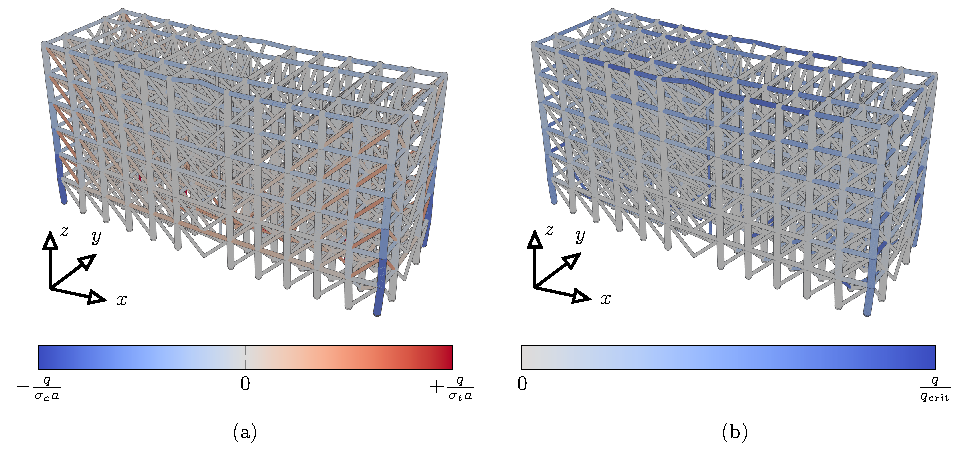
\includegraphics[width=\linewidth]{figures/05_cellular_opt/00_module_scale_failure/12x4x6_mech.pdf}
        \caption{Stress (a-c) and local buckling (b-d) failure criteria plotted on the monolithic and the 12x4x6-3x3x3 cases.}
        \label{fig:05_scale_failure}
    \end{figure}

\paragraph{Influence of the complexity of the module}
We now shift our focus to another parameter of modular structures: the module complexity, defined as the number of candidate members $\bar{n}$ inside a module. To understand how this parameter influences the optimized structures, we set up an analysis similar to the one previously conducted for the module scale. Utilizing the same test case, we divide the structure into 6x2x3 submodules along the X, Y, and Z axes, respectively. We discretize each module using a 2x2x2, a 3x3x3, a 4x4x4, and a 5x5x5 fully connected ground structure ($\bar{n}=28$, $\bar{n}=351$, $\bar{n}=2016$ , $\bar{n}=7750$, rispectively). The same analysis is conducted on a 12x4x6 structure to validate the test on a different modular structure.


\begin{table*}
    \centering
    \small
    \begin{tabular}{lx{1.4cm}x{1.4cm}x{1.4cm}x{1.4cm}x{1.4cm}x{1.4cm}x{1.4cm}x{1.4cm}}
        \toprule
        \multirow{2}{*}{\textbf{Quantity}} & \multicolumn{4}{l}{6x2x3} & \multicolumn{3}{l}{12x4x6} \\ \cmidrule(lr){2-5} \cmidrule(lr){6-8} 
     & 2x2x2      & 3x3x3     &  4x4x4    &  5x5x5    &   2x2x2      & 3x3x3        & 4x4x4      \\
     &  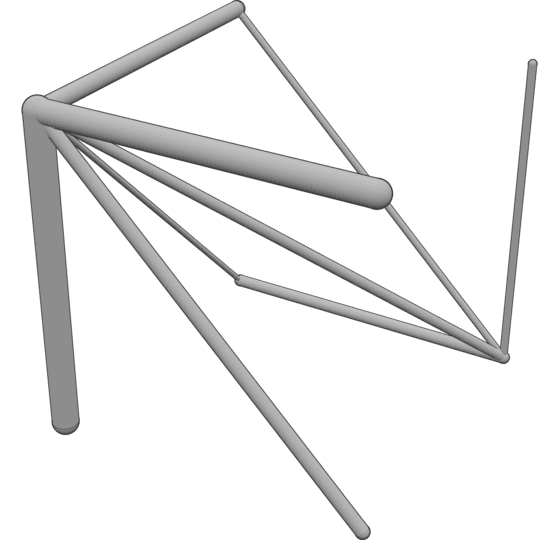
\includegraphics[width=1.3cm]{figures/05_cellular_opt/00_module_complexity_cell/6x2x3_2x2x2_c.png}    &  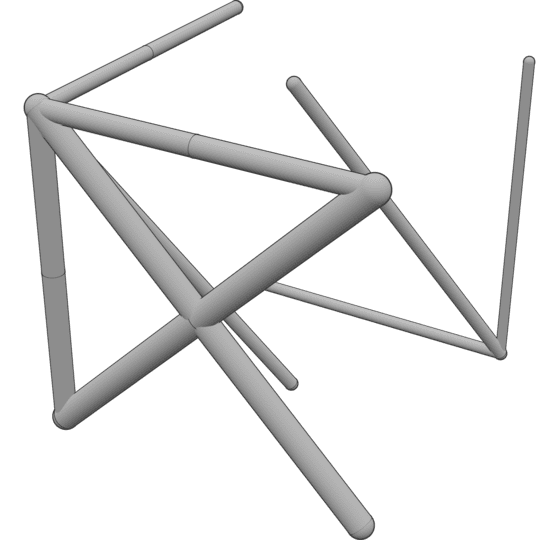
\includegraphics[width=1.3cm]{figures/05_cellular_opt/00_module_complexity_cell/6x2x3_3x3x3_c.png}    & 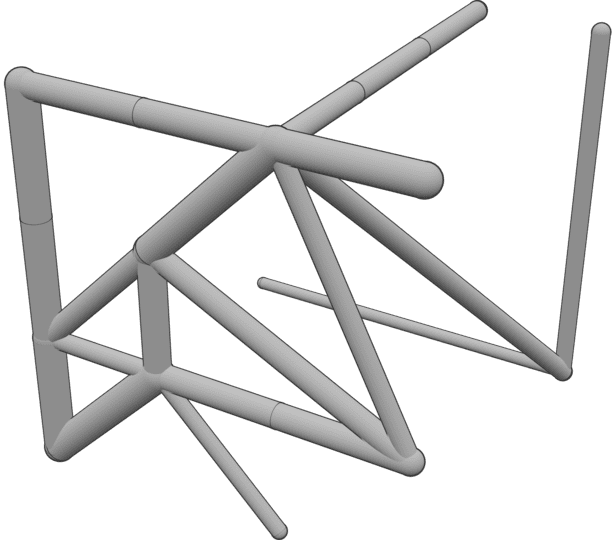
\includegraphics[width=1.3cm]{figures/05_cellular_opt/00_module_complexity_cell/6x2x3_4x4x4_c.png}     & 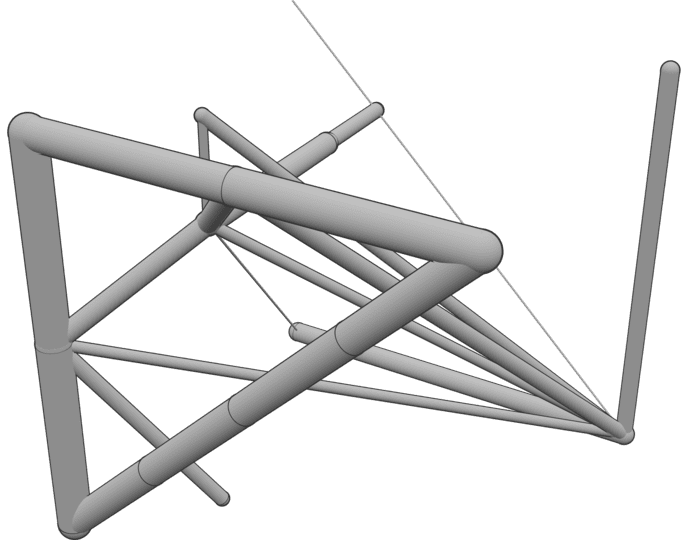
\includegraphics[width=1.3cm]{figures/05_cellular_opt/00_module_complexity_cell/6x2x3_5x5x5_c.png}     & 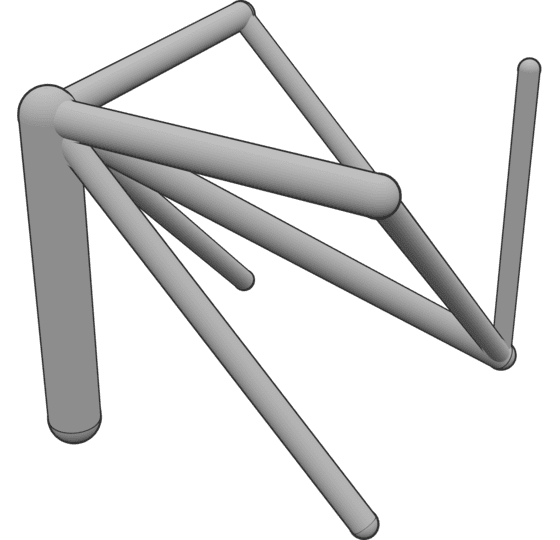
\includegraphics[width=1.3cm]{figures/05_cellular_opt/00_module_complexity_cell/12x4x6_2x2x2_c.png}        & 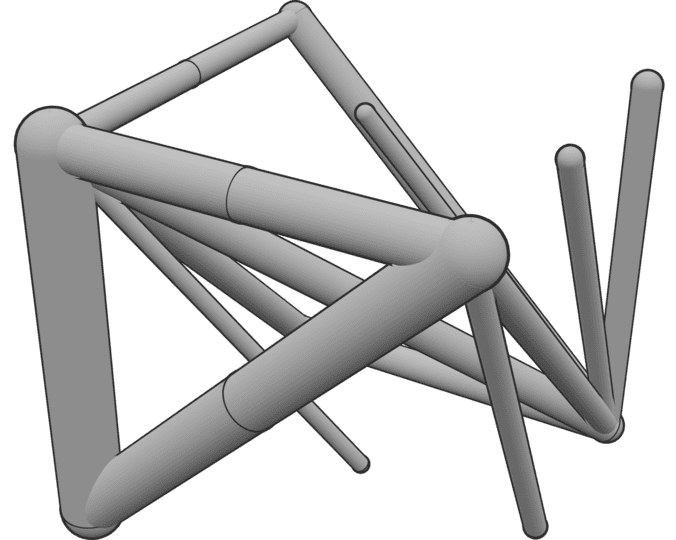
\includegraphics[width=1.3cm]{figures/05_cellular_opt/00_module_complexity_cell/12x4x6_3x3x3_c.png}   &  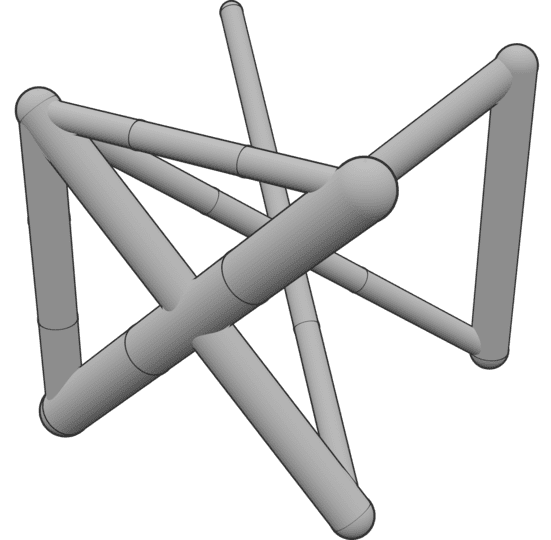
\includegraphics[width=1.3cm]{figures/05_cellular_opt/00_module_complexity_cell/12x4x6_4x4x4_c.png}      \\
    $\bar{n}_\text{opt}\;(\bar{n})$ &  9 (28) &   19 (351)   &  88  (2016)   &  88 (7750)    &   9 (28)   &    15 (351)        &   22   (2016)  \\
    $N_\text{sub}$           &    36  &   36   &   36   &   36   &    288     &   288      &    288    \\
    $N_\text{opt}\;(N_\text{el})$  &  324 (1008) &  468 (12636)   & 792  (72576)   & 792 (279000)     & 2592 (8064)     &   4320   (101088)       &  6336 (580608)     \\
    $V$ [\unit{cm^3}] & 27.074 & 24.323     & 17.098     & 17.083     &  70.559    &  65.723       & 60.368       \\
    $V$ [\unit{\percent}] &4.812&4.324&3.040&3.036&12.544&11.684&10.732        \\
    C [\unit{J}]      & 4.22     &   3.63   & 4.49     & 3.91     &   3.35      &  1.84       & 2.43       \\
    $a_\text{max}$ [\unit{mm^2}]      & 9.40     &   5.33   &   3.39   &  3.77    &  5.45       &   2.60      &   2.97    \\
    $\varphi$   &\qty{14.81}{\percent}&\qty{20.51}{\percent}&\qty{12.12}{\percent}&\qty{20.20}{\percent}&\qty{1.85}{\percent}&\qty{1.46}{\percent}&\qty{1.32}{\percent}         \\
    $\psi$& 0.446    &   0.327   & 0.414     & 0.419     &   0.178      &  0.127       & 0.136       \\
    t        & \hms{0;0;6}  &  \hms{0;5;42} & \hms{0;14;20} & \hms{3;17;00} & \hms{0;0;48} & \hms{0;42;50} &  \hms{32;4;00}      \\ \bottomrule
    \end{tabular}
    \caption{Numeric results of the parametric study on the influence of the module complexity on the optimized structures.}
    \label{tab:05_comp_results}
    \end{table*}

The results of the parametric study are presented in a tabular format in \tabref{tab:05_comp_results}, along with the rendering of the module. Once again, we have plotted the most interesting aspects separately. The first aspect we examine is how the volume of the optimized structure is influenced by the module complexity $\bar{n}$. In \figref{fig:05_comp_v}, we observe that an increase in $\bar{n}$ generally has a beneficial effect on volume. However, this effect becomes less pronounced as complexity increases, and in this particular test case, the volume reduction stagnates after the module complexity reaches 4x4x4.

Regarding computational time (see \figref{fig:05_comp_t}), we notice a relationship similar to the one already observed for the submodule scale. The computational time goes up as the module complexity increases. This is understandable because, unlike the case with the number of subdomains, in this scenario, the number of design variables increases along with the number of candidates and, consequently, the constraints.

The 3D renderings of the optimized structures for the 6x2x3 submodules case are presented in \figref{fig:05_comp_results}, allowing the reader to observe the evolution of the module's topology toward greater complexity (from $\bar{n}_\text{opt}=9$ to $\bar{n}_\text{opt}=88$ for the 2x2x2 and 5x5x5 cases, respectively). While in low complexity, the optimizer prioritizes tensile elements, in more complex cases, we observe the apparition of shorter elements less influenced by local buckling.


\begin{figure*}
    \hspace*{\fill}
    \subcaptionbox{}{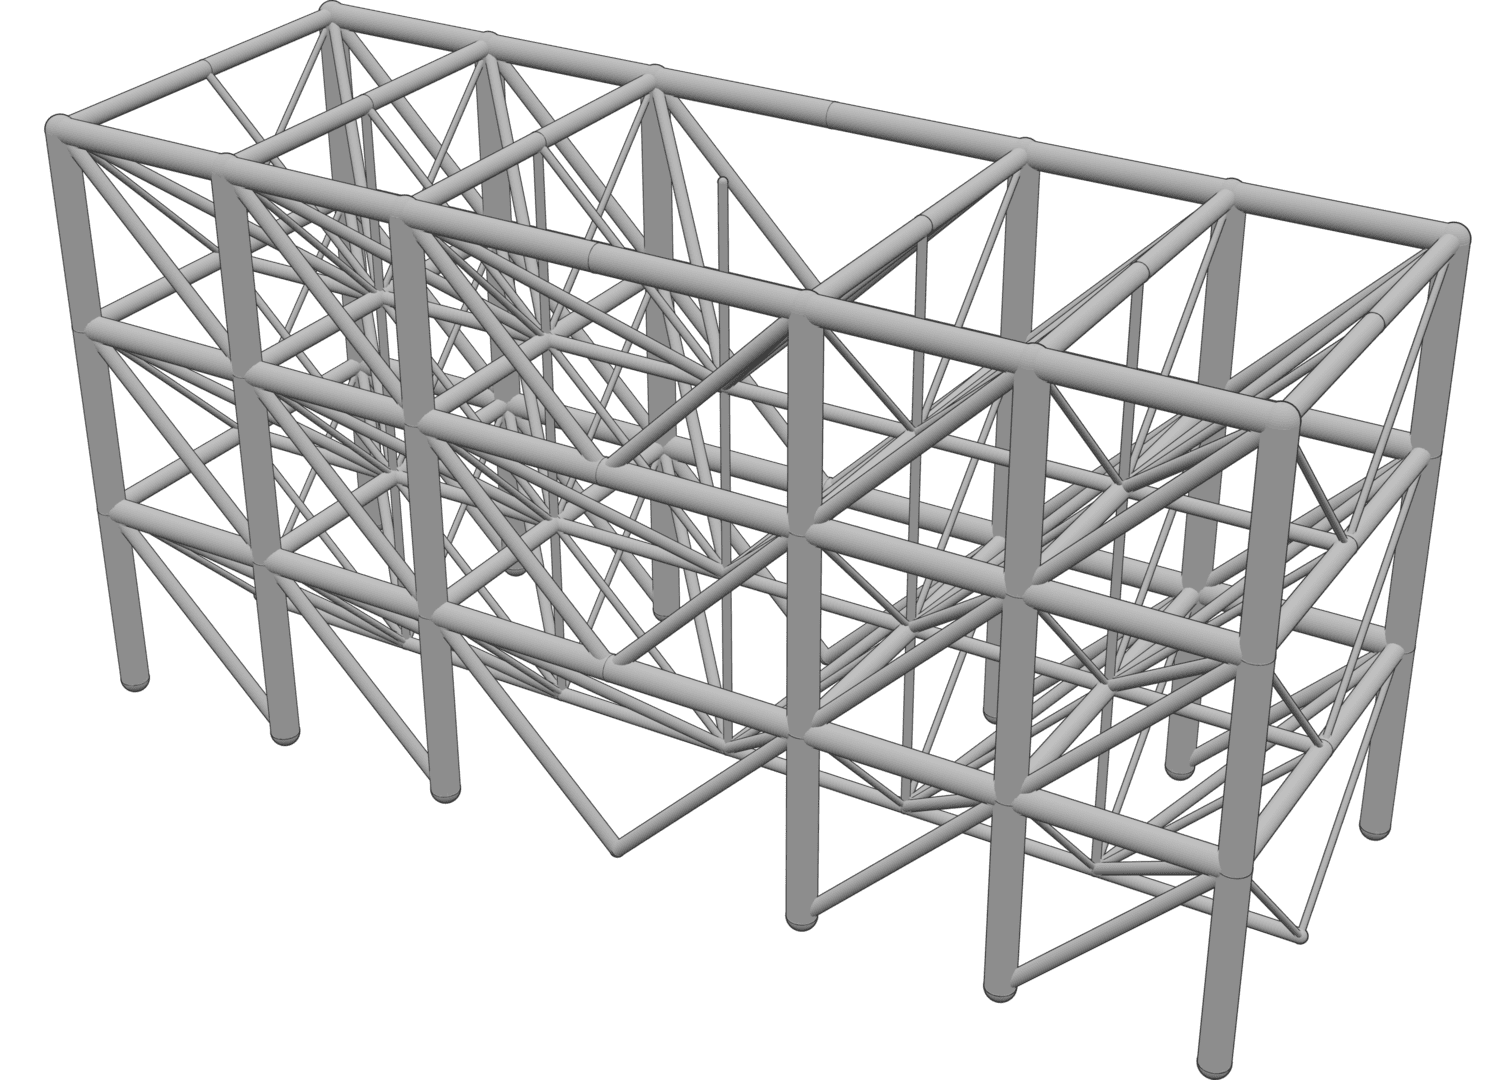
\includegraphics[width=0.23\linewidth]{figures/05_cellular_opt/00_module_complexity/6x2x3_2x2x2.png}}
    \hfill
    \subcaptionbox{}{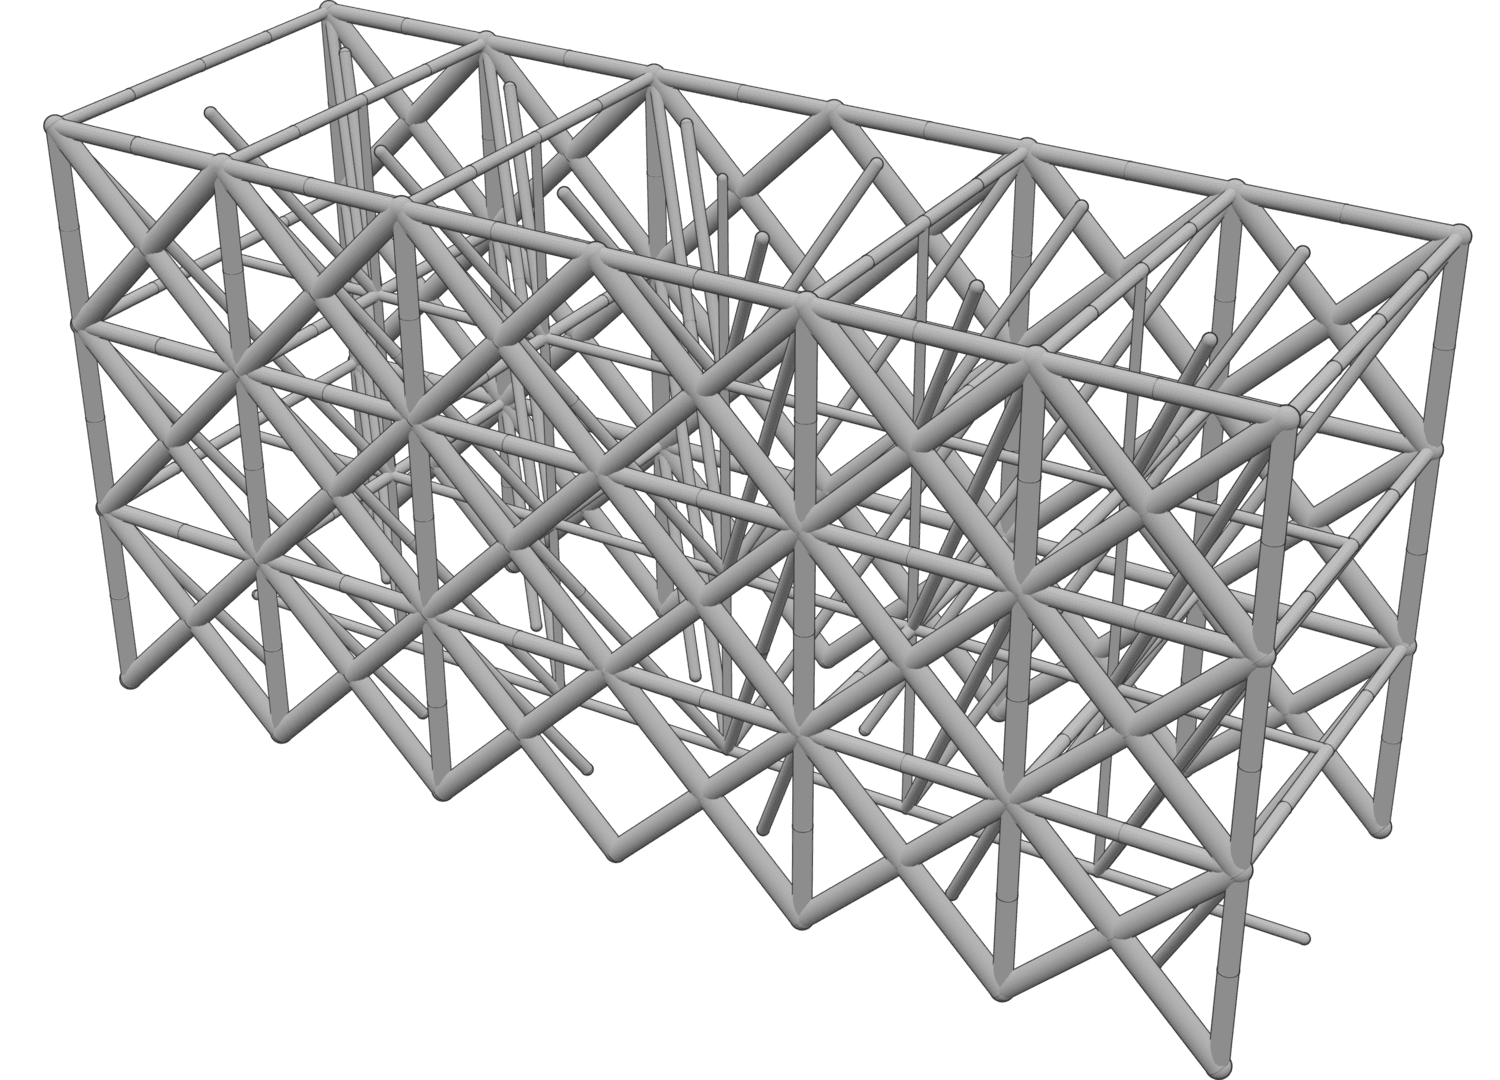
\includegraphics[width=0.23\linewidth]{figures/05_cellular_opt/00_module_complexity/6x2x3_3x3x3.png}}
    \hfill
    \subcaptionbox{}{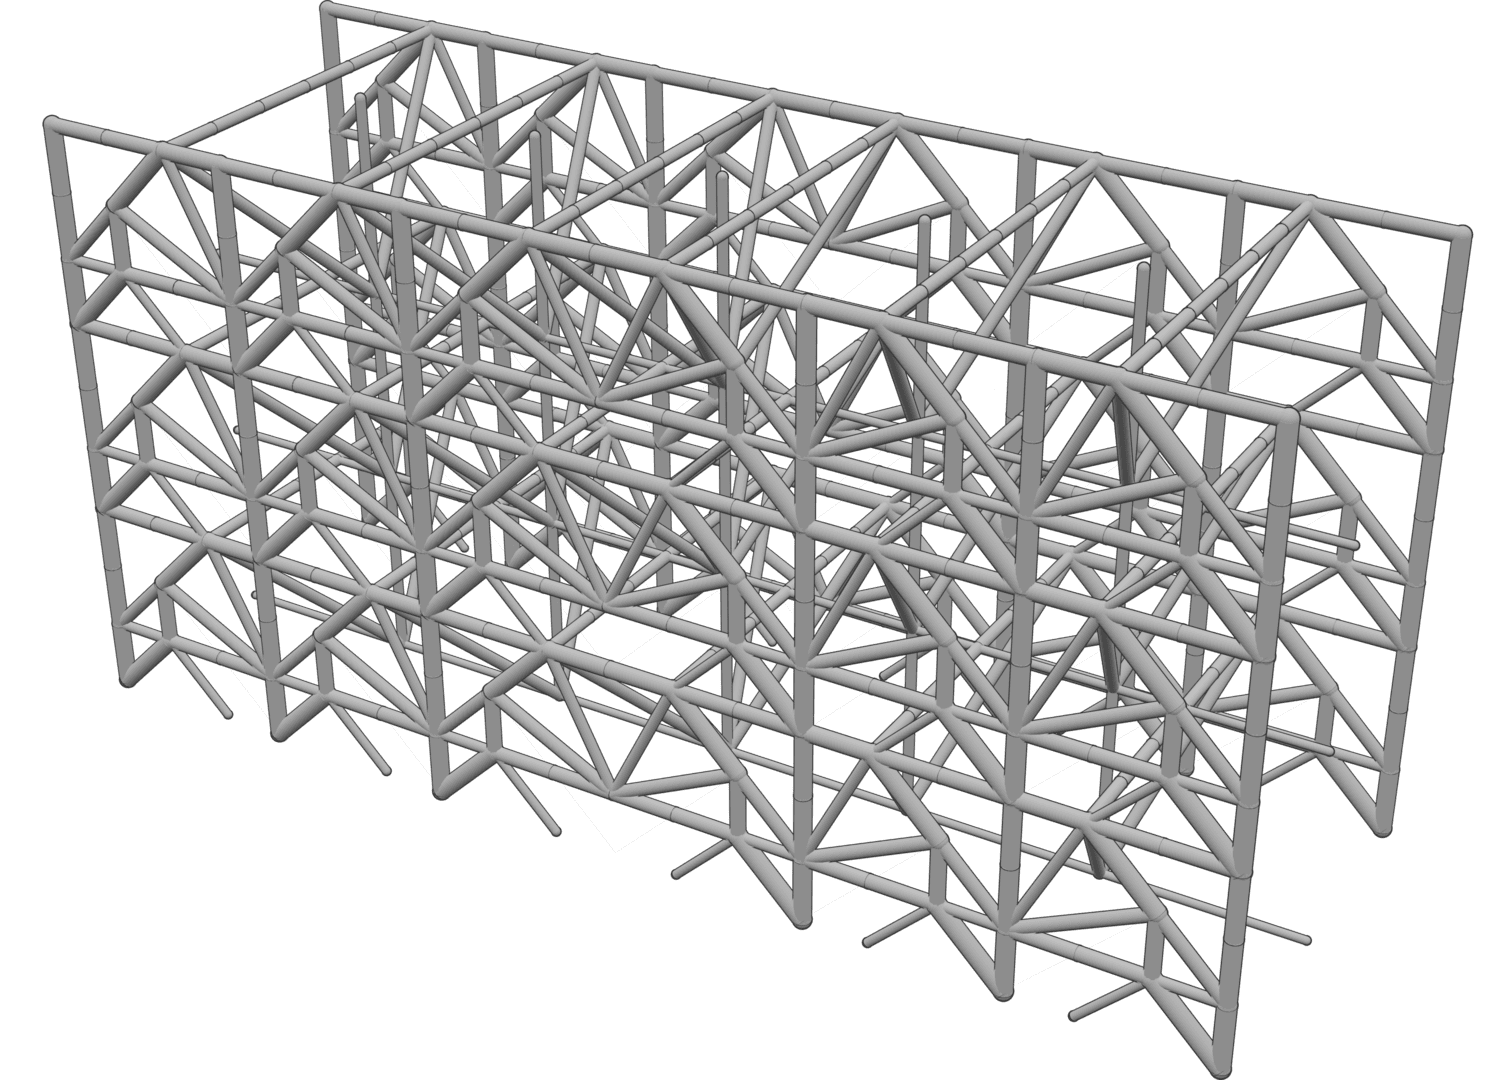
\includegraphics[width=0.23\linewidth]{figures/05_cellular_opt/00_module_complexity/6x2x3_4x4x4.png}}
    \hfill
    \subcaptionbox{}{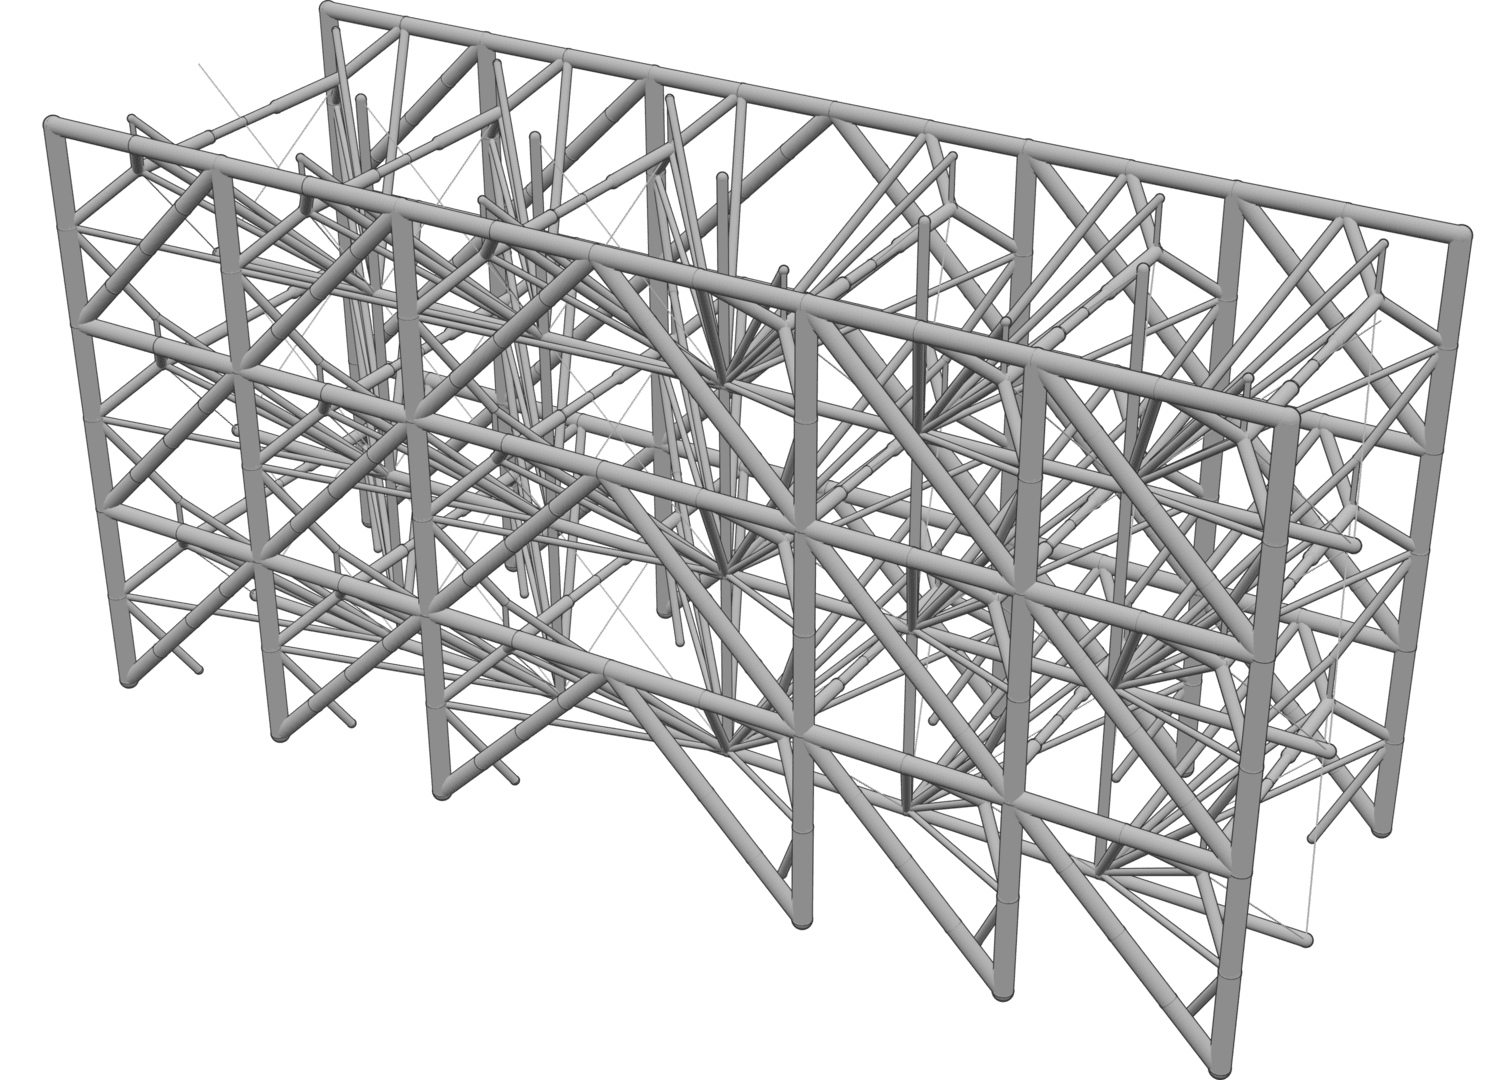
\includegraphics[width=0.23\linewidth]{figures/05_cellular_opt/00_module_complexity/6x2x3_5x5x5.png}}
    \hspace*{\fill}
    \bigskip
    \hspace*{\fill}
    \subcaptionbox{}{\includegraphics[width=0.23\linewidth]{figures/05_cellular_opt/00_module_complexity/6x2x3_2x2x2_XZ.png}}
    \hfill
    \subcaptionbox{}{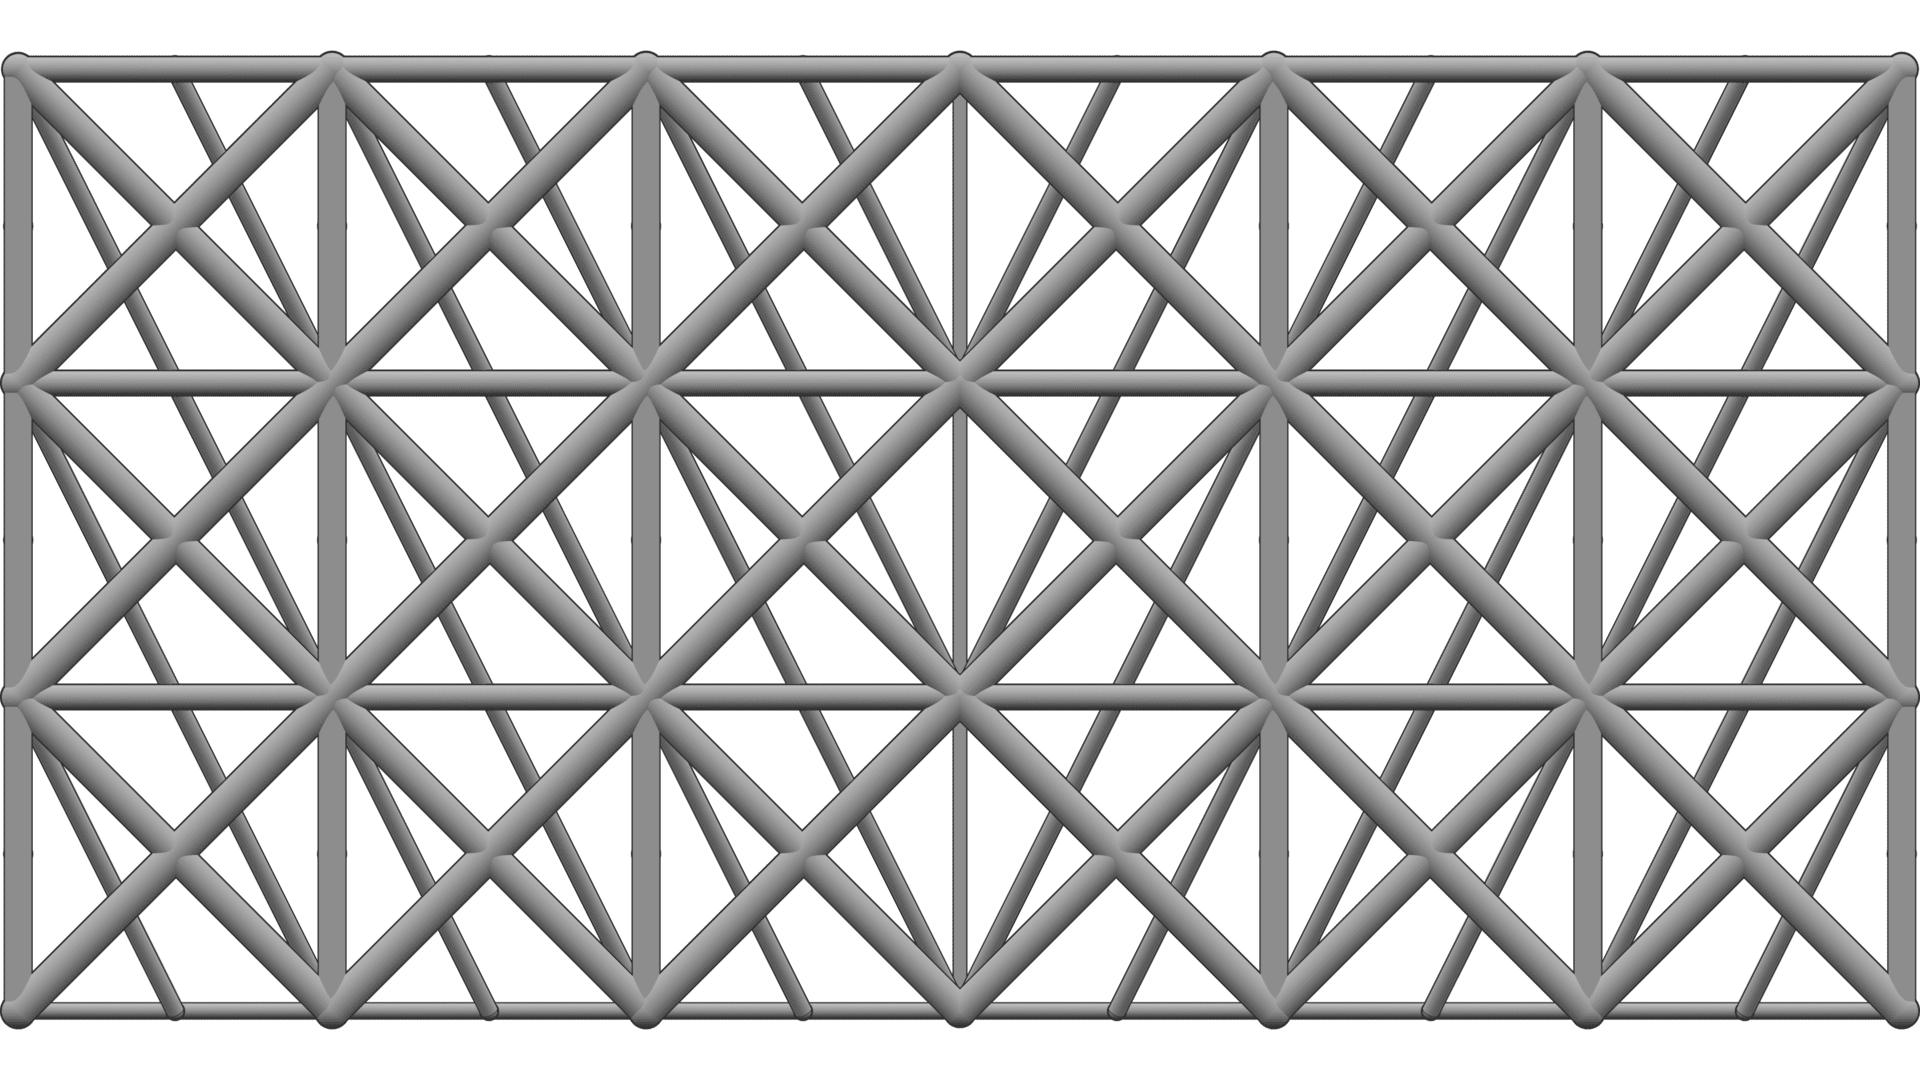
\includegraphics[width=0.23\linewidth]{figures/05_cellular_opt/00_module_complexity/6x2x3_3x3x3_XZ.png}}
    \hfill
    \subcaptionbox{}{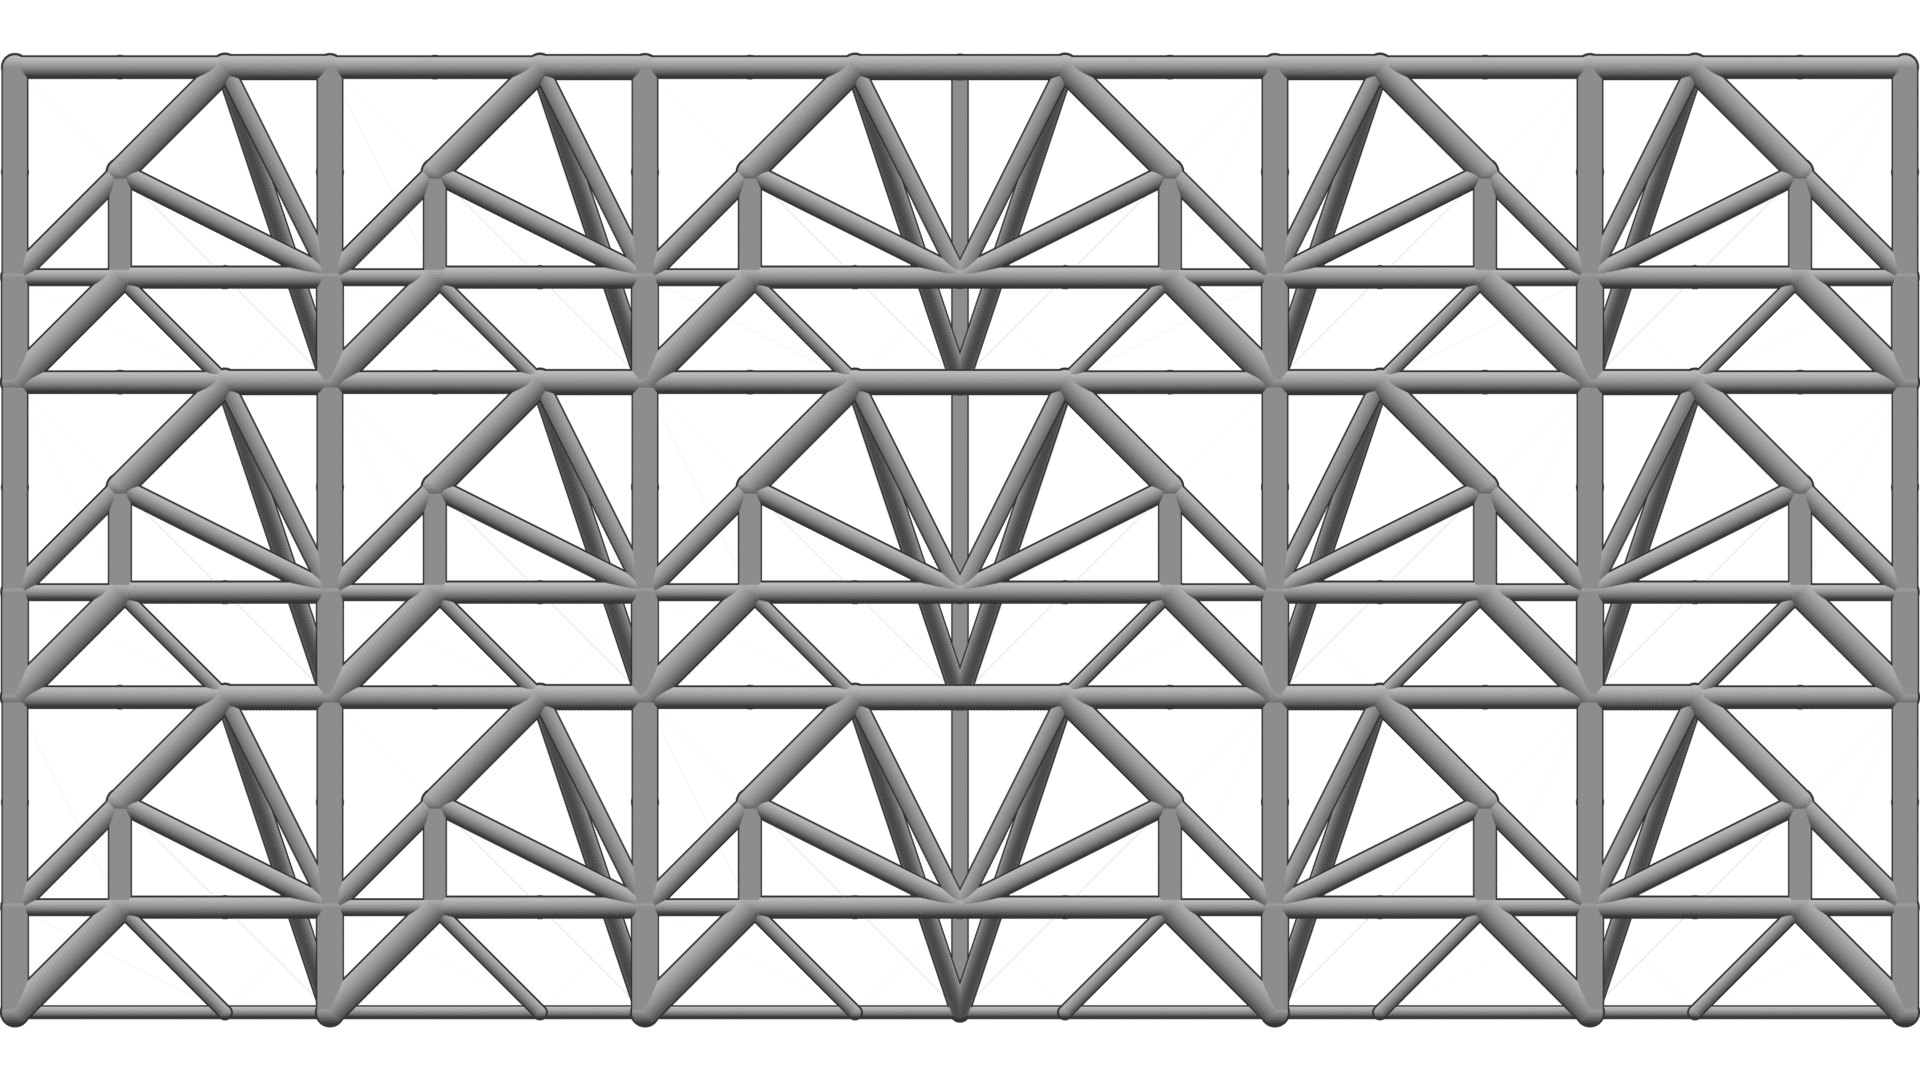
\includegraphics[width=0.23\linewidth]{figures/05_cellular_opt/00_module_complexity/6x2x3_4x4x4_XZ.png}}
    \hfill
    \subcaptionbox{}{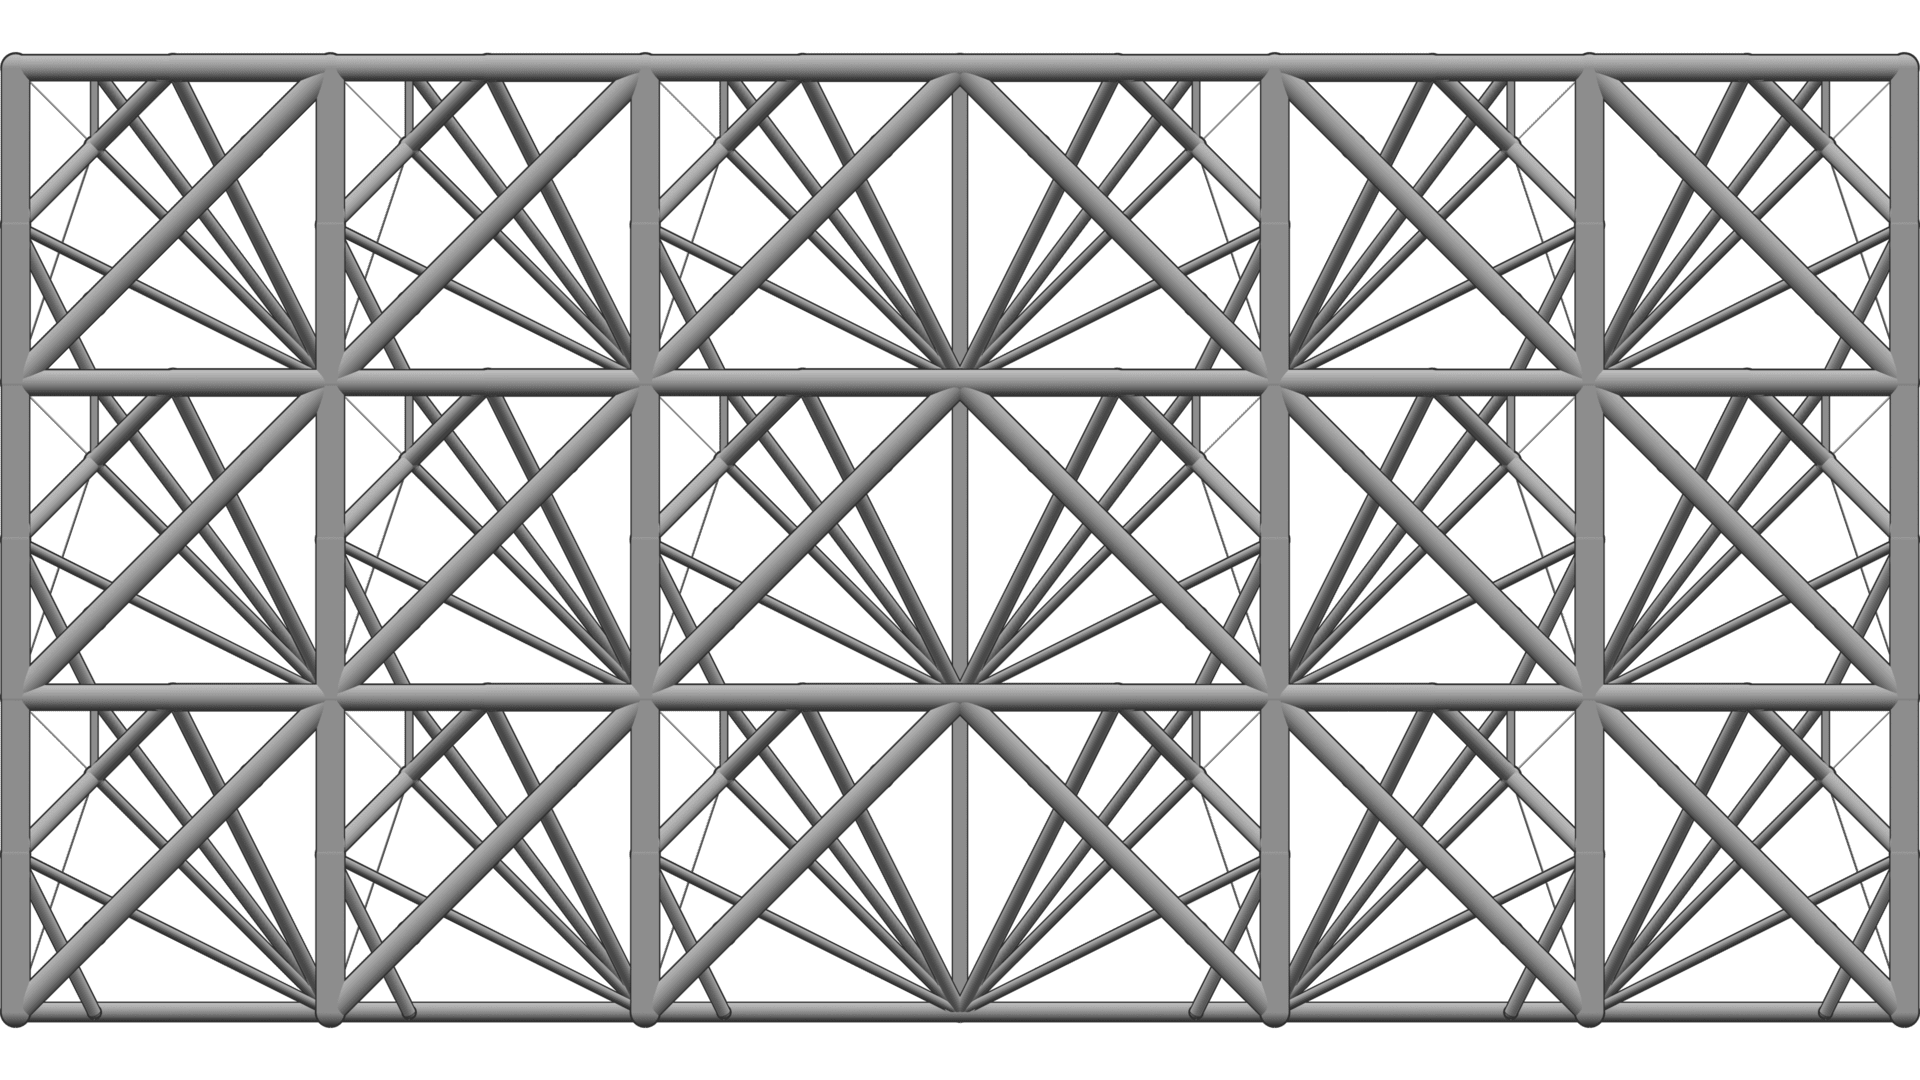
\includegraphics[width=0.23\linewidth]{figures/05_cellular_opt/00_module_complexity/6x2x3_5x5x5_XZ.png}}
    \hspace*{\fill}
    \caption{Rendering of the optimized structures with 2x2x2 (a-e), 3x3x3 (b-f), 4x4x4 (c-g), and 5x5x5 (d-h) module complexity. The number of subdomains is 6x2x3.}
    \label{fig:05_comp_results}
\end{figure*}

\begin{marginfigure}
    \centering
    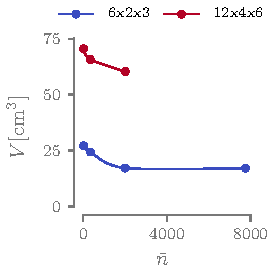
\includegraphics{figures/05_cellular_opt/00_module_complexity_tab/comp_tab_v.pdf}
    \caption{Influence of the module complexity on the volume of the optimized modular structure.}
    \label{fig:05_comp_v}
\end{marginfigure}

\begin{marginfigure}
    \centering
    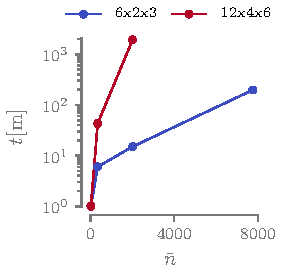
\includegraphics{figures/05_cellular_opt/00_module_complexity_tab/comp_tab_t.pdf}
    \caption{Influence of the module complexity on the computational time of the optimization.}
    \label{fig:05_comp_t}
\end{marginfigure}

\begin{marginfigure}
    \centering
    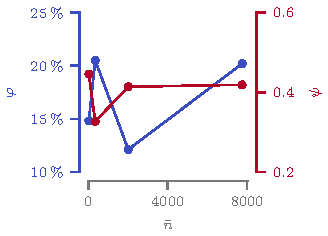
\includegraphics[width=\linewidth]{figures/05_cellular_opt/00_module_complexity_tab/comp_tab_param.pdf}
    \caption{Influence of the module complexity on the loading metrics $\varphi$ and $\psi$ of the optimized structures.}
    \label{fig:05_comp_param}
\end{marginfigure}

It is interesting to note that the number of active bars in the optimized structure is quite dependent on the complexity of the module. However, in this specific case, we see that it saturates at $\bar{n}=88$ in the 6x2x3 case, suggesting that we have reached the convergence of the discretization.

Finally, in \figref{fig:05_comp_param}, we present the numerical values of $\varphi$ and $\psi$. Unlike our earlier observations, the trends of these parameters are not monotonic and do not follow an explicit trend. While these indices aid in understanding how much a truss is loaded, they don't necessarily provide clear hints on optimality. A structure loaded to the maximum of the material contributes to achieving a lighter design but is not sufficient, as this example demonstrates.

\paragraph{Design of experiments}
With the data gathered thus far, we aim to construct the \gls{doe} for optimized modular structures. The objective is to monitor how the outcomes vary by introducing a change in the preconditions, represented by one or more independent variables. In our case, the chosen independent variables are the number of subdomains $N_\text{sub}$ ($x_1$) and module complexity $\bar{n}$ ($x_2$), while the observed responses are the total structural volume $V$ and the computational time $t$. For simplicity, we continue to limit ourselves to cubic cells.

We have chosen to use a quadratic model with interaction (the term $x_1x_2$) in an attempt to capture a potential interference between $x_1$ and $x_2$, represented as follows:
\begin{equation}
    a\:x_1^2+b\:x_2^2+c\:x_1x_2+d\:x_1+e\:x_2+f
\end{equation}
The coefficients are determined by solving a least squares system using the data presented earlier in this section.

\begin{margintable}
    \small
    \centering
    \sisetup{table-auto-round}
    \begin{tabular}{cS[table-number-alignment = center, table-format = 1.2e1]}
    \toprule
    \textbf{Coeff.} & {\textbf{Value}} \\ \midrule
    $a$ & 9.002e-08    \\
    $b$ &  -1.022e-05   \\
    $c$ &  -1.770e-06   \\
    $d$ &  -2.644e-03   \\
    $e$ &   1.011e-01  \\
    $f$ &   2.881e+01  \\
    \bottomrule
    \end{tabular}
    \caption{Coefficients of the quadratic function used to model how the volume $V$ varies with the number of subdomains $N_\text{sub}$ and the module complexity $\bar{n}$.}
    \label{tab:05_doe_coeff_v}
\end{margintable}

\begin{margintable}
    \small
    \centering
    \sisetup{table-auto-round}
    \begin{tabular}{cS[table-number-alignment = center, table-format = 1.2e1]}
    \toprule
    \textbf{Coeff.} & {\textbf{Value}} \\ \midrule
    $a$ & 1.547e-03    \\
    $b$ & -2.871e-04    \\
    $c$ &  2.896e-01   \\
    $d$ &  -2.084e+01   \\
    $e$ &  -5.543e+00   \\
    $f$ & 0    \\
    \bottomrule
    \end{tabular}
    \caption{Coefficients of the quadratic function used to model how the computational time $t$ varies with the number of subdomains $N_\text{sub}$ and the module complexity $\bar{n}$.}
    \label{tab:05_doe_coeff_t}
\end{margintable}

We present the outcomes of the \gls{doe} in \figref{fig:05_doe} for the structure volume $V$. In the upper part of the image, we display the surface response along with a scatter plot of the optimized structures (a), and additionally, the isovalue lines plot (b). It is noticeable that the volume $V$ is strongly influenced by the number of subdomains $N_\text{sub}$, as indicated by the horizontal orientation of the isovalue lines. This suggests that the steepest gradient of the function is in the vertical direction. Less voluminous modular structures tend to be structures with fewer subdomains characterized by high complexity $\bar{n}$. However, when examining subfigures (c) and (d), representing the surface response for computational time $t$ , it is evident that high module complexity $\bar{n}$ is associated with an elevated computational time.

The coefficients of the quadratic model are given in \tabref{tab:05_doe_coeff_v} and \tabref{tab:05_doe_coeff_t} for the volume and computational time, respectively. We see that for the volume the coefficient that defines the most the behavior of the response surface is $e$, the coefficient that relates to the linear term for the number of subdomains. The interaction between the two independent variables -- the coefficient $c$ -- is low, showing that the two variables do not add up when modified together. This is not true for the computation time, where the interaction coefficient is relevant, together with the two linear terms. Once again, the quadratic coefficients $a$ and $b$ are less important, suggesting in general a linear response.

The coefficients of the quadratic model are presented in \tabref{tab:05_doe_coeff_v} and \tabref{tab:05_doe_coeff_t} for the volume and computational time, respectively. Notably, for the volume $V$, the coefficient that predominantly influences the behavior of the response surface is $e$, which corresponds to the linear term for the number of subdomains $N_\text{sub}$. The interaction coefficient between the two independent variables, denoted as $c$, is low, indicating that the two variables do not significantly contribute when modified together. This is in contrast to computational time, where the interaction coefficient is relevant, along with the two linear terms. In the two cases, the quadratic coefficients $a$ and $b$ are relatively less important, suggesting a generally linear response.

\begin{figure*}
    \hspace*{\fill}
    \subcaptionbox{}{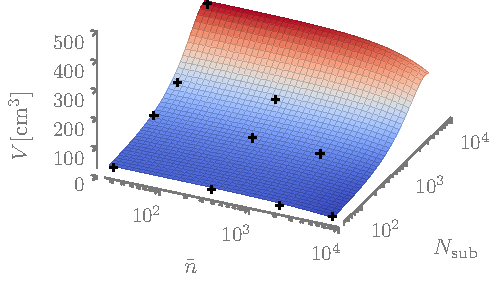
\includegraphics{figures/05_cellular_opt/00_doe_vol/doe_vol.pdf}}
    \hfill
    \subcaptionbox{}{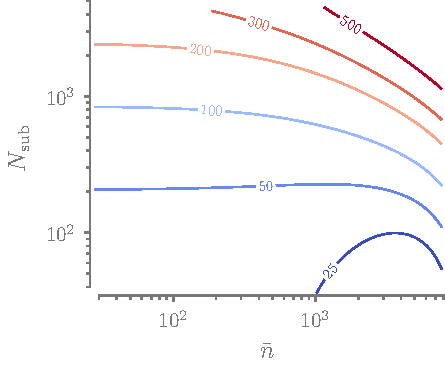
\includegraphics{figures/05_cellular_opt/00_doe_vol/doe_vol_cont.pdf}}
    \hspace*{\fill}
    \bigskip
    \hspace*{\fill}
    \subcaptionbox{}{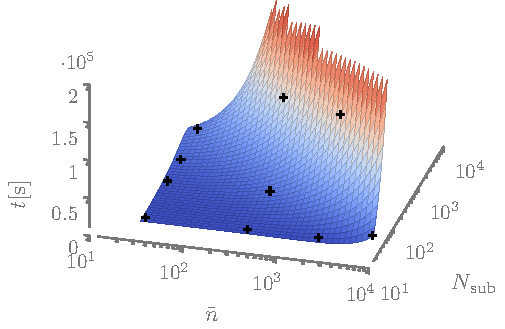
\includegraphics{figures/05_cellular_opt/00_doe_time/doe_time.pdf}}
    \hfill
    \subcaptionbox{}{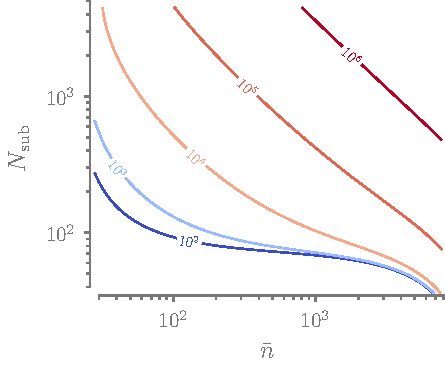
\includegraphics{figures/05_cellular_opt/00_doe_time/doe_time_cont.pdf}}
    \hspace*{\fill}
    \caption{\acrfull{doe} response curves and isocurves plot for the volume (a-b) and computational time (c-d).}
    \label{fig:05_doe}
\end{figure*}

Finally, we present the main effects plot for the volume and module complexity in \figref{fig:05_doe_main_eff}. The concept is to plot, for each factor or interaction, the effect (summed with the overall mean) as a function of the level. The advantage of this representation is to offer an immediate visualization of the various effects.
\begin{figure}
    \centering
    \subcaptionbox{}{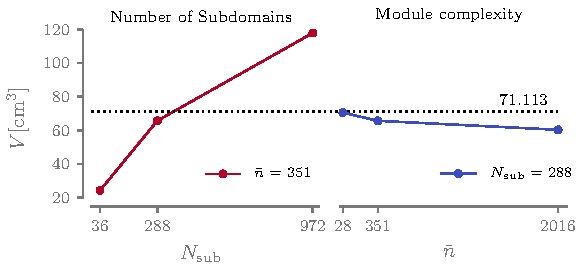
\includegraphics{figures/05_cellular_opt/00_doe_main_effect_plots/tab_v.pdf}}
    \bigskip
    \subcaptionbox{}{\includegraphics{figures/05_cellular_opt/00_doe_main_effect_plots/tab_t.pdf}}
    \caption{Main effects plot of volume (a) and computational time (b).}
    \label{fig:05_doe_main_eff}
\end{figure}
\paragraph{Discussion on the DOE}
We can utilize this \gls{doe} as a tool to give general recommendations. While the specific numeric values and their magnitudes just found are tailored to the presented example, we assume that the observed trends are generally correct and applicable to modular structures as a whole. Therefore, we can conclude that in scenarios where minimizing mass is the primary objective, aiming for the fewest possible number of subdomains is preferred. However, additional constraints must be considered. For example, having fewer subdomains implies an increase in the physical size of individual submodules. Yet, there is often a manufacturing maximum size that restricts this increase. Consequently, the recommendation is to achieve the largest possible subdomains that can be produced within the limitations of the chosen manufacturing technology.

Although higher complexity significantly impacts computational time, its influence on optimization outcomes is not substantial. Therefore, opting for a medium complexity, such as 3x3x3 nodes in the module (or 4x4 in 2D), strikes a balance between computational cost and optimization effectiveness.

\subsection{Comparison with the optimized octet-truss}
The proposed modular \gls{tto} algorithm is benchmarked against one of the most popular cell topologies found in the literature: the octet-truss (see \figref{fig:05_octet_module}). The octet-truss is a cell known for its highly effective mechanical properties, achieving about half the theoretical values of the upper Hashin-Shtrikman bounds~\sidecite{deshpande_effective_2001} for isotropic materials.

To conduct the benchmark, the simply supported 3D beam is divided into 6x2x3 and 12x4x6 cubic subdomains, which are then populated with the octet-truss topology. The cross-sectional areas of the cell members are all equal, and the numerical value is determined by performing a parametric optimization. The octet-truss structure is constrained by stress, local buckling, and kinematic compatibility constraints for every member of the structure. The optimization is performed using Altair OptiStruct.


\begin{marginfigure}
    \centering
    \includegraphics[width=0.7\linewidth]{figures/05_cellular_opt/00_octet/05_Cell__Topology_NLP_iso.png}
    \caption{Rendering of a single octet-truss module.}
    \label{fig:05_octet_module}
\end{marginfigure}

\begin{figure*}
    \hspace*{\fill}
    \subcaptionbox{}{\includegraphics[width=0.46\linewidth]{figures/05_cellular_opt/00_octet_truss_comp_6/octet.png}}
    \hfill
    \subcaptionbox{}{\includegraphics[width=0.46\linewidth]{figures/05_cellular_opt/00_octet_truss_comp_6/6x2x3_3x3x3.png}}
    \hspace*{\fill}
    \bigskip
    \hspace*{\fill}
    \subcaptionbox{}{\includegraphics[width=0.46\linewidth]{figures/05_cellular_opt/00_octet_truss_comp_6/octet_XZ.png}}
    \hfill
    \subcaptionbox{}{\includegraphics[width=0.46\linewidth]{figures/05_cellular_opt/00_octet_truss_comp_6/6x2x3_3x3x3_XZ.png}}
    \hspace*{\fill}
    \bigskip
    \hspace*{\fill}
    \subcaptionbox{}{\includegraphics[width=0.46\linewidth]{figures/05_cellular_opt/00_octet_truss_comp_12/octet.png}}
    \hfill
    \subcaptionbox{}{\includegraphics[width=0.46\linewidth]{figures/05_cellular_opt/00_octet_truss_comp_12/12x4x6_3x3x3.png}}
    \hspace*{\fill}
    \bigskip
    \hspace*{\fill}
    \subcaptionbox{}{\includegraphics[width=0.46\linewidth]{figures/05_cellular_opt/00_octet_truss_comp_12/octet_XZ.png}}
    \hfill
    \subcaptionbox{}{\includegraphics[width=0.46\linewidth]{figures/05_cellular_opt/00_octet_truss_comp_12/12x4x6_3x3x3_XZ.png}}
    \hspace*{\fill}
    \caption{Comparison of the octet-truss structures (a-c-e-g) and the TTO structures (b-d-f-h) for two differnet numbers of submodules, 6x2x3 and 12x4x6.}
    \label{fig:05_octet_results}
\end{figure*}

\figref{fig:05_octet_results} displays the 3D rendering of the two optimized octet-truss structures (left part of the image) compared to the modular \gls{tto} structures (right part of the image). It is noticeable how the \gls{tto} algorithm guides the topology of the module toward higher efficiency, creating vertical columns loaded in compression that support thin wires loaded in tension. On the other hand, the octet-truss topology is fixed and exhibits quasi-isotropic mechanical behavior. The octet-truss is a module with good homogenized elastic properties in all directions, thanks to its numerous planes of symmetry. It is, thus, less suitable for structural applications where all the subdomains experience similar loading conditions. In such cases, the module will be equally stiff and strong in every direction, not aligned with the principal stress directions.

We notice that in the octet-truss structure, there are no members orientated exactly along the $z$ axis, while in the \gls{tto} optimized cell, they are the most massive. This tells us that this is the most efficient direction to put the material to get a strong cell. On top of that, the upper and lower faces of the cell present a cross design (see \figref{fig:05_octet_module}) that works well for torque but not for tension and compression loading. A new study exploring what happens if we rotate the cell could be interesting.

\begin{table}
    \centering
    \small
    \begin{tabular}{lx{1.4cm}x{1.4cm}x{1.4cm}x{1.4cm}}
        \toprule
        \multirow{2}{*}{\textbf{Quantity}}         &\multicolumn{2}{l}{6x2x3} & \multicolumn{2}{l}{12x4x6} \\ 
             \cmidrule(lr){2-3} \cmidrule(lr){4-5} 
     &Octet& 3x3x3      & Octet     &  3x3x3    \\
    $N_\text{sub}$       &36& 36&288&288   \\
    $N_\text{opt}\;(N_\text{el})$ &1008& 468 (12636)&7488&4320 (101088) \\
    $V$ [\unit{cm^3}]& 65.752 & 24.323&121.038&65.723         \\
    $V$ [\unit{\percent}] &11.692&4.324&21.524&11.684         \\
    C [\unit{J}]    &1.67&3.63&1.12&1.84         \\
    $a_\text{max}$ [\unit{mm^2}]    & 3.69 &  5.33&1.83&2.60         \\ 
    $\varphi$    &\qty{0.39}{\percent}&\qty{20.51}{\percent}&\qty{0.05}{\percent} & \qty{1.46}{\percent}        \\
    $\psi$    &0.075&0.327&0.026&0.127         \\ \bottomrule
    \end{tabular}
    \caption{Numerical results of the comparison between octet-truss and TTO structures.}
    \label{tab:05_octet_results}
    \end{table}

The numerical results are presented in \tabref{tab:05_octet_results} and confirm our observations. The volume of the octet-truss structures is approximately three times and twice the volume of the modular \gls{tto} optimized structures for the 6x2x3 and the 12x4x6 test cases, respectively. This significant gap between the two types of structures is also evident when examining the values of $\varphi$ and $\psi$. These values drop to very low levels because the cross-sectional value of the entire structure is determined by the value at which a bar on the structure becomes critical. For these structures, only four bars are critical (due to symmetry). Better results could have been obtained by providing more design freedom to the optimization of the octet-truss, using multiple cross-sectional design variables, but this approach has not been taken here. It is important to note that the comparison presented here does not account for the weight of fasteners and joints necessary to link the cells together.

\subsection{Using multiple module topologies}
We have explored two extremes so far -- the fully modular and the monolithic structures. Now, we aim to investigate the scenarios in between. Up to this point, our study on modular structures has been limited to a single topology of the module, \ie, $N_\text{T}=1$. This is because, when dealing with multiple module topologies, another crucial question arises: how to optimize the module layout? How should the modules be arranged in the structure to minimize the overall volume of the part? This critical question will be discussed in-depth later in the thesis. For now, as we begin to consider multiple module topologies, we make a significant simplification by determining the layout based solely on good engineering common sense, without an additional optimization process.

\begin{figure}
    \centering
    \includegraphics[width=0.6\linewidth]{figures/05_cellular_opt/00_mutiple_bc/supported_3D_symm.pdf}
    \caption{Graphical representation of the given module layout for the simply supported 3D beam.}
    \label{fig:05_mutiple_bc}
\end{figure}

Let us reconsider the simply supported 3D beam divided into a grid of 6x2x3 subdomains. This time, we optimize the structure using three different modules $N_\text{T}=3$. The modules are discretized using an equal fully connected ground structure with 3x3x3 nodes. The module mapping matrix of the structure is provided as an input for the optimization\sidenote{The module mapping matrix is $\matr{H}=
\begin{bmatrix}
    1 & 0 & 0\\
    1 & 0 & 0\\
    1 & 0 & 0\\
    0 & 0 & 0\\
    0 & 1 & 0\\
    0 & 1 & 0\\
    0 & 1 & 0\\
    0 & 0 & 1\\
    0 & 0 & 1\\
    0 & 0 & 1\\
\end{bmatrix}$}
and it represents the module layout shown in \figref{fig:05_mutiple_bc}. 

The optimized structure features an interesting design made by two elongated spars that support multiple tensile members responsible for carrying the given loads. The spars exhibit a design that favors long tensile members, interconnected by compressive bars. The resulting optimized structure is illustrated in Figure \ref{fig:05_multiple_topology_sol}.

We now examine the modules of the optimized structure. Firstly, we observe that the optimizer sets all the cross-sectional areas of module $t=2$ to zero, judging it as unimportant for the mass optimization of the structure. This highlights the importance of considering the possibility of an empty topology when optimizing the module layout in the structure. Secondly, we note instances where the module is composed of bars that are disconnected \eg in $t=0$, potentially necessitating additional post-processing for obtaining a manufacturable design.

\begin{figure*}
    \centering
    \includegraphics{figures/05_cellular_opt/00_multiple_topology/support_sol.pdf}
    \caption{Orthographic views of the topology of the optimized modular simply supported 3D beam. (a) XZ plane (b) YZ plane (c) XY plane (d) auxiliary perspective view.}
    \label{fig:05_multiple_topology_sol}
\end{figure*}

\begin{marginfigure}
    \centering
    \includegraphics[width=\linewidth]{figures/05_cellular_opt/00_multiple_tab/multi_tab.pdf}
    \caption{Comparison of the volume and computational time of the structure with multiple modules with the monolithic and the fully modular structures.}
    \label{fig:05_multiple_topology_sol_graph}
\end{marginfigure}

\begin{figure}
    \centering
    \includegraphics[width=\linewidth]{figures/05_cellular_opt/00_multiple_failure/mul_mech.pdf}
    \caption{Stress (a-c) and local buckling (b-d) failure criteria plotted on the multiple and single module modular structures.}
    \label{fig:05_multiple_topology_sol_mech}
\end{figure}

The optimized structure with $N_\text{T}=3$ is now compared to the reference monolithic structure and the 6x2x3-3x3x3 structure with $N_\text{T}=3$ to assess the difference in mechanical performance due to the increased number of modules. The results are presented in \tabref{tab:05_multiple_topology_sol}. Interestingly, the computational time of the $N_\text{T}=1$ solution is lower $(t = \hms{00;3;22}$) compared to the $N_\text{T}=3$ structure $(t = \hms{00;5;42}$). This comes as a surprise, considering that the $N_\text{T}=1$ optimization problem involves more design variables (as three times the number of cross-sectional areas are optimized). However, it turns out that having more design freedom makes the optimization process easier, as the constraints are more straightforward to satisfy. The trends of the volume and computational time are illustrated graphically in \figref{fig:05_multiple_topology_sol_graph}.

The volume reduction is attributed to a more efficient utilization of the subdomains' topology, which now varies with the subdomain position. This can be observed by examining the more efficient use of material, with a greater number of bars reaching the mechanical failure limit ($\varphi = 61.90\%$ for $N_\text{t} = 3$ compared to $\varphi = 61.90\%$ for $N_\text{t} = 1$) and, in general, a more uniform structure loading ($\psi = 0.716$ vs. $\psi = 0.327$). The stress and buckling failure criteria are shown in \figref{fig:05_multiple_topology_sol_mech} for further insight.


\begin{table}
    \centering
    \small
    \begin{tabular}{lx{1.4cm}x{1.4cm}x{1.4cm}x{1.4cm}x{1.4cm}}
        \toprule
        \multirow{2}{*}{\textbf{Quantity}}   & 7x3x4 & \multicolumn{3}{l}{6x2x3-3x3x3-$N_\text{T}=3$} & 6x2x3 3x3x3 $N_\text{T}=1$ \\ \cmidrule(lr){2-2} \cmidrule(lr){3-5} \cmidrule(lr){6-6} 
     & --      & $t=0$    &  $t=1$    &  $t=2$    &   $t=0$       \\
     & --  &  \includegraphics[width=1.3cm]{figures/05_cellular_opt/00_multiple_cell/05_Cell_000_Topology_NLP_iso.png}    & \includegraphics[width=0.85cm]{figures/05_cellular_opt/00_multiple_cell/05_Cell_001_Topology_NLP_iso.png}     & --  & \includegraphics[width=1.3cm]{figures/05_cellular_opt/00_module_complexity_cell/6x2x3_3x3x3_c.png} \\
     $\bar{n}_\text{opt}\;(\bar{n})$ &1984 &   10 (351)   &  18  (351)       &   -- (351)   &    19 (351)  \\
    $N_\text{sub}$           &    1  & \multicolumn{3}{c}{36}   &    36    \\
    $N_\text{opt}\;(N_\text{el})$ &20 (1984) &  \multicolumn{3}{c}{336 (12636)}     &  468 (12636)     \\
    $V$ [\unit{cm^3}]&9.907 &  \multicolumn{3}{c}{12.032}   & 24.323       \\
    $V$ [\unit{\percent}] &1.761& \multicolumn{3}{c}{2.139} &4.324       \\
    C [\unit{J}]    &3.71     & \multicolumn{3}{c}{6.14}  & 3.63       \\
    $a_\text{max}$ [\unit{mm^2}]   &37.61   &  \multicolumn{3}{c}{7.13}   &   5.33    \\
    $\varphi$    &\qty{100.00}{\percent}&\multicolumn{3}{c}{\qty{61.90}{\percent}}&\qty{20.51}{\percent}        \\
    $\psi$    &1.000&\multicolumn{3}{c}{0.716}&0.327          \\ 
    t     &\hms{0;0;4}  & \multicolumn{3}{c}{\hms{00;3;22}} &  \hms{00;5;42}      \\ \bottomrule
    \end{tabular}
    \caption{Numerical results of the comparison between the structure with multiple modules with the monolithic and the fully-modular structures. }
    \label{tab:05_multiple_topology_sol}
    \end{table}
    
    This study suggests that employing more modules for optimization allows the achievement of less voluminous structures, potentially approaching the performance of monolithic structures. However, this introduces a compromise between volume (and consequently mass) and the ease of manufacturing, a topic we will delve into further in the upcoming chapter.

\section{Conclusion}
In this chapter, we introduced a modular structure optimization algorithm based on the \acrfull{tto} and variable linking. Initially, we investigated the impact of modularity constraints on the topological buckling phenomenon and sensitivity analysis. Subsequently, we adapted the two-step optimization algorithm with reinitialization presented in Chapter~\ref{chp:04} to solve the proposed modular formulation.

The modular \gls{tto} algorithm is then tested on multiple two- and three-dimensional test cases. Initially, we observe an equivalence between modular structures and structures loaded with multiple load cases. The utilization of a repeating module throughout the structure significantly impacts the volume, as the module needs to perform well under various loading conditions concurrently. Subsequently, we conducted an extensive parametric analysis of the number of subdomains and module complexity. Based on the results of the \acrfull{doe}, we provide recommendations: fewer subdomains are generally preferable, with the module as large as manufacturably possible. Module complexity plays a role in volume minimization but has a relatively low impact. Finally, the modular \gls{tto} structures are benchmarked against one of the most commonly used module topologies in the literature: the octet-truss lattice.

At the end of the chapter, we conducted a final optimization using multiple module topologies. The incorporation of multiple modules, some of which may have an entirely empty topology, emerged as a crucial factor that contributes to the reduction of modular structure volume. This approach allows modular structures to approach the volume of monolithic structures while offering additional ease of manufacturing. However, the utilization of multiple modules raises a new question: how are the modules arranged within the different subdomains of the structure?